% Tento soubor nahraďte vlastním souborem s obsahem práce.
%=========================================================================
% Autoři: Michal Bidlo, Bohuslav Křena, Jaroslav Dytrych, Petr Veigend a Adam Herout 2019
\chapter{Úvod}

Blockchain je distribuovaný systém, ktorý nachádza využitie v~aplikáciách elektronických mien (kryptomien), zmenární, volieb a podobných systémov s~požiadavkou na vysokú bezpečnosť. Tradičné systémy pre tieto typy aplikácií poskytujú bezpečnosť založenú na centrálnej dôveryhodnej autorite. Na proti tomu, blockchain je decentralizovaný a jeho bezpečnosť je vystavaná na kryptografickom dôkaze. Kapitola~\ref{chap:blockchain} popisuje podrobnejšie túto technológiu a jej vlastnosti.

Distribuovaný a decentralizovaný systém ako je blockchain musí poskytovať protokol pomocou, ktorého sa všetci jeho užívatelia bezpečne zhodnú na rovnakom stave. Takýto protokol sa nazýva konsenzus. Táto práca sa zaoberá skupinou protokolov, ktoré uznášajú konsenzus metódou Proof-of-Stake. Princípom tohoto dôkazu je, že vlastníci veľkého podielu zdrojov uložených v~blockchaine sú najdôveryhodnejší užívatelia. Kapitola~\ref{chap:consenzus} rozoberá najbežnejšie typy konsenzus protokolov ako aj známe útoky na ich bezpečnosť.

Cieľom tejto práce je posúdiť tri zvolené Proof-of-Stake protokoly z~hľadiska bezpečnosti a výkonnosti. Kapitola~\ref{chap:harmony} analyzuje protokol Harmony, ktorého cieľom je poskytnúť vysokú škálovatelnosť. Kapitola~\ref{chap:solana} sa zaoberá protokolom Solana, ktorý je zameraný na vysokú priepustnosť transakcií. Kapitola~\ref{chap:ouroboros} popisuje protokol Ouroboros, ktorý si kladie za cieľ formálne dokázať svoju bezpečnosť. Kapitola~\ref{chap:protocol-comparison} sumarizuje vlastnosti všetkých troch protokolov a porovnáva ich z~hľadiska rôznych aspektov.

Zvolené tri protokoly budú simulované z~hľadiska bezpečnosti a výkonnosti. Kapitola~\ref{chap:simulators-overview} poskytuje prehľad existujúcich simulátorov blockchainu. V~rámci tejto kapitoly je vykonané porovnanie najvhodnejších nástrojov a je zvolený jeden, ktorý bude ďalej rozšírený o~podporu troch zvolených protokolov (Harmony, Solana a Ouroboros).

Na záver sú v~kapitole~\ref{chap:summary} zhrnuté aktuálne výsledky tejto práce vzhľadom k~stanoveným cieľom.

\chapter{Blockchain}\label{chap:blockchain}

Táto kapitola vysvetľuje základné koncepty a pojmy spojené z~technológiou blockchain, ako aj samotnú dátovú štruktúru blockchain. Sekcia~\ref{sec:ladger} vysvetľuje pojmi distribuovaná účtovná kniha a blockchain. Ďalej rozoberá vlastnosti a využitie blockchainu. Sekcia~\ref{sec:crypto} vysvetľuje kryptografiu používanú v~blockchaine (hashovanie, a asymetrická kryptografia). Sekcia~\ref{sec:p2p} popisuje peer-to-peer siete a ich využitie v~blockchaine. Na záver sú v~sekcii~\ref{sec:data-struct-blockchain} spojené všetky vysvetlené koncepty dokopy a je popísaná samotná dátová štruktúra blockchain.

\section{Distribuovaná účtovná kniha}\label{sec:ladger}
\textit{Účtovná kniha} (anglicky \textit{ledger}) sa v~histórii ľudstva dlhodobo používa na záznam rôznych položiek, najčastejšie peňazí a majetku. Príchod digitalizácie a globalizácie presunul tento známy koncept z~papierovej podoby do elektronickej. Toto prináša nové výzvy z~hľadiska bezpečnosti.
\textit{Distribuovaná účtovná kniha} (anglicky \textit{distributed ledger}) je všeobecne technológia, ktorá poskytuje dôveryhodnú a bezpečnú databázu zdieľanú naprieč viacerými inštitúciami, krajinami a to typicky verejne. Veľmi bežným odvetvím využitia distribuovanej účtovnej knihy je bankovníctvo. Banka poskytuje centralizovanú autoritu, ktorá zabezpečuje bezpečnú manipuláciu s~peniazmi klientov. Tento koncept označujeme ako centralizovaná účtovná kniha.~\cite{dltUkReport}

V~roku 2008 bola publikovaná práca~\cite{satoshiBitcoin}, ktorá navrhla \textit{decentralizovanú} distribuovanú účtovnú knihu. Práca navrhla koncept elektronického platobného systému, ktorého bezpečnosť je založená na kryptografickom dôkaze namiesto dôvere v~centralizovanú autoritu. Takáto distribuovaná účtovná kniha sa nazýva \textbf{blockchain} (ďalej \textbf{BC}).
\subsection{Vlastnosti BC}
BC je dátová štruktúra, ktorá má nasledujúce vlastnosti~\cite{zhengBlockchainOverview}:
\begin{itemize}
	\item \textbf{Decentralizácia} (anglicky \textit{decentralization}): BC funguje nad peer-to-peer sieťou, ktorá nepotrebuje centralizovanú dôveryhodnú autoritu, ale na zabezpečenie konzistencie používa konsenzus protokol.
	\item \textbf{Auditovateľnosť} (anglicky \textit{auditability}): BC v~sebe nesie celú histórie zmien dátového obsahu a teda každú zmena stavu dát uložených v~BC je možné sledovať.
	\item \textbf{Nemennosť} (anglicky \textit{persistency}): Modifikácia alebo zmazanie časti dátového obsahu BC nie je možná.
	\item \textbf{Anonymita} (anglicky \textit{anonymity}): Užívatelia pracujúci s~BC používajú na identifikáciu asymetrickú kryptografiu s~digitálnym podpisom. Takýto kryptografický identifikátor neodhaľuje skutočnú identitu užívateľa a pritom umožňuje nepopierateľne určiť vlastníka elektronického zdroja.
\end{itemize}

Tieto vlastnosti BC sú zabezpečené pomocou peer-to-peer siete na ktorej je BC postavený (viď sekcia~\ref{sec:p2p}) a taktiež pomocou samotnej dátovej štruktúry, ktorá využíva modernú kryptografiu (viď sekcia~\ref{sec:data-struct-blockchain}).~\cite{horizenAcademy}

\subsection{Aplikačné využitie}

BC bol navrhnutý a po prvýkrát implementovaný za účelom poskytnúť elektronickú peňažnú menu nezávislú od centralizovaného bankovníctva. Tento prvý a najznámejší BC je Bitcoin~\cite{satoshiBitcoin}. Avšak vlastnosti BC technológie nachádzajú uplatnenie vo veľkom množstve odvetví. Nasledujúci zoznam vymenúva niekoľko aplikácií, ktoré BC môže riešiť~\cite{homoliakBlockchain}:

\begin{itemize}
	\item \textbf{Elektronická peňaženka}: Elektronické peňaženky pre obchod s~nejakou formou digitálnych peňazí (typicky v~podobe tokenov). Takéto tokeny sú vlastnené pomocou privátneho kľúča, ktorý má uschovaný majiteľ. Ten môže vlastníctvo tokenov presúvať na iné subjekty v~danej sieti.
	\item \textbf{Zmenárne}: V~dnešnej dobe existuje veľké množstvo elektronických peňažných mien postavených nad BC. Takéto meny všeobecne označujeme ako kryptomeny. Z~dôvodu veľkého množstva kryptomien sa prirodzene zvyšuje dopyt po zmenárni medzi jednotlivými kryptomenami. Klasická zmenáreň je riešená tradične centralizovanou autoritou. Avšak BC je vhodnou technológie aj pre decentralizovanú zmenáreň.
	\item \textbf{Súborové systémy}: V~dnešnej dobe už existujú decentralizované súborové systémy založené na peer-to-peer sieťach. Implementácia takéhoto decentralizovaného súborového systému ako BC by nám umožnila nepopierateľne a trasovateľne verzovať zmeny v~obsahu.
	\item \textbf{Správa identít}: Táto služba je typicky zabezpečovaná centrálnou autoritou, ktorá prideľuje pre konkrétne entity určité zdroje na ktoré majú právo. Ide o~schému podobnú banke. BC by v~tomto prípade opäť umožnil náhradu tejto centralizovanej autority za decentralizovanú sieť.
	\item \textbf{Voľby}: Elektronické hlasovanie je ďalším vhodným príkladom, kde sa dá efektívne využiť BC. Hlasujúce entity predstavujú decentralizovanú sieť a vlastnosti BC zase poskytujú transparentnosť a verejnú overiteľnosť.
	\item \textbf{Reputačné systémy}: Tieto služby merajú úroveň dôvery v~určité entity. Typickým príkladom je reputácia rôznych predajcov na základe hlasovania zákazníkov. Transparentnosť a nemennosť BC histórie by znížila možnosť manipulácie s~reputáciu v~prospech nejakej entity.
	\item \textbf{Aukcie}: Elektronická aukcia je služba veľmi podobná elektronickej peňaženke alebo zmenárni s~podobnými bezpečnostnými požiadavkami. Tieto vlastnosti by opäť dokázala pokryť technológia BC.
\end{itemize}

\section{Viacvrstvová abstrakcia BC}

Existuje veľké množstvo BC protokolov, ktoré majú rôzne využitie a technologické riešenie. Avšak všetky tieto implementácie sú založené na spoločnom koncepte distribuovanej účtovnej knihy. Pre ich jednotnú klasifikáciu použijeme nasledujúci model abstrakcie so štyrmi vrstvami~\cite{homoliakBlockchain}:

\begin{enumerate}
	\item \textbf{Sieťová vrstva} predstavuje najnižšiu vrstvu abstrakcie a zaoberá sa peer-to-peer sieťou. Sieť rieši pripájanie nových peerov a komunikácia medzi uzlami v~sieti (šírenie transakcií a blokov). Táto vrstva má kritický dosah na výkonnosť BC. Napríklad, verejný BC ako je Bitcoin tvorí veľmi rozsiahlu sieť s~tisíckami aktívnych uzlov. V~takejto sieti sa už vlastnosti ako stratovosť dát alebo priepustnosť nezanedbateľne prejaví na rýchlosti a stabilite celého BC. Sieťová vrstva je popísaná v~sekcii~\ref{sec:p2p}.~\cite{fanPerfEval}
	\item \textbf{Konsenzus vrstva} definuje protokol pomocou, ktorého sa ustanovuje dohoda na stave BC. Konsenzus v~BC je popísaný v~kapitole~\ref{chap:consenzus}.
	\item \textbf{Dátová vrstva} (alebo tiež úložisko) definuje model transakcií (binárny hashovací strom, hashovacie a kryptografické algoritmy). Sekcia~\ref{sec:crypto} popisuje kryptografické primitíva používané v~technológii BC a sekcia~\ref{sec:data-struct-blockchain} popisuje BC ako dátovú štruktúru.
	\item \textbf{Aplikačná vrstva} definuje využitie v~konkrétnej službe (napríklad kryptomena).
\end{enumerate}

\section{Peer-to-peer sieť}\label{sec:p2p}

Technológia BC je postavená na peer-to-peer sieťach. Peer-to-peer sieť sa podieľa na decentralizovanosti, nemennosti a auditovateľnosti BC. 

Peer-to-peer sieť je dynamický súbor nezávislých uzlov (anglicky \textit{peers}), ktoré sú prepojené do grafu. Každý uzol obsahuje zdroje, ktoré zdieľa všetkým ostatným uzlom v~sieti.~\cite{p2pBuford, p2pSchollmeier} Dôvod existencie peer-to-peer sietí je teda decentralizovaný spôsob zdieľania zdrojov ako sú súbory, fyzické zariadenia, výpočtový výkon alebo aj elektronické finančné zdroje. Dnes existuje množstvo peer-to-peer sietí. Veľmi známe sú napríklad Gnutella, Kazaa alebo BitTorrent.~\cite{p2pEssence}

\subsection{Referenčný model}
Najbežnejšie technické riešenie peer-to-peer siete je navrstvenie siete (anglicky \textit{overlay network}) na už existujúcu sieť, ktorou je typicky Internet. Takúto sieť potom môžeme definovať ako päticu $(P,R,I,F_P,F_R)$, kde:
\begin{itemize}
	\item $P$ je množina uzlov
	\item $R$ je množinu zdrojov
	\item $I$ je priestor identifikátorov
	\item $F_P: P \rightarrow I$ je funkcia, ktorá mapuje uzoly na identifikátory
	\item $F_R: R \rightarrow I$ je funkcia, ktorá mapuje zdroje na identifikátory
\end{itemize}

Obrázok~\ref{img:p2p-ref-model} ukazuje princíp fungovania takto definovanej siete. Tvorba siete s~týmto modelom je potom závislá od šiestich návrhových aspektov:
\begin{enumerate}
	\item Voľba priestoru identifikátorov.
	\item Mapovanie zdrojov a uzlov na identifikátory.
	\item Správa priestoru identifikátorov v~réžii uzlov siete.
	\item Tvorba grafu (štruktúra siete).
	\item Stratégia smerovania (anglicky \textit{routing}).
	\item Stratégia údržby.
\end{enumerate}
Konkrétne riešenie pre popisovaných šesť aspektov je zavislé od požiadaviek na efektivitu, škálovateľnosť, samoorganizovateľnosť, odolnosť voči chybám a kooperáciu.~\cite{p2pEssence}

\subsection{Využitie v~BC}\label{subsec:bc-usage}

Peer-to-peer sieť umožňuje BC uchovávať jeho obsah decentralizovane a pritom bezpečne. Tento koncept si vysvetlíme na prípade BC, ktorý sa využíva ako kryptomena.

Elektronické financie sú typicky reprezentované pomocou elektronických mincí. Takáto minca je definovaná nejakou unikátnou sekvencie bitov. Avšak narozdiel od fyzických mincí, elektronické mince umožňujú jednoduchú falzifikáciu. Útočník skopíruje bitový reťazec danej mince a zaplatí ním viacnásobne rôzne produkty. Tento útok sa volá zdvojnásobenia výdavkov (anglicky \textit{double-spending attack}). Proti tomuto útoku existuje tradičné zabezpečenie pomocou centrálnej autority. Banka je centrálna autorita, ktorá schvaľuje všetky manipulácie s~elektronickými mincami a teda neumožní použiť mincu takýmto podvodným spôsobom. Avšak toto riešenie nie je možné použiť v~decentralizovanej sieti, kde centrálna autorita neexistuje. V~prípade decentralizovanej siete je možné zabrániť tomuto útoku pomocou použitia peer-to-peer siete v~kombinácii s~BC.~\cite{doubleSpending}

Kryptomena Bitcoin ako prvá navrhla použitie peer-to-peer siete v~spojení s~BC technológiou pre zabránenie double-spending útoku. V~takejto sieti je jediný zdroj na zdieľanie a to je dátová štruktúra BC v~ktorej sú uložené všetky informácie o~elektronických financiách. Zjednodušene môžeme povedať, že majorita uzlov siete zdieľa rovnaký zdroj (rovnakú kópiu BC). Ak chce niektorý uzol vykonať finančnú transakciu tak zašle správu s~navrhovanou zmenou BC do siete. Uzly v~tejto sieti nie je potrebné identifikovať pretože správy posielané v~tejto sieti nie sú smerované na žiadne konkrétne miesto. Keď uzol prijme správu s~nejakou modifikáciu tak si overí či ide o~validnú požiadavku na finančnú transakciu. Štruktúra BC používa modernú kryptografiu na overenie validnosti transakcie (pozri sekciu~\ref{sec:crypto}). BC vlastnený väčšinou siete je ten, ktorý sa považuje za pravdu. Útočník by musel teda vlastniť aspoň 51\,\% uzlov v~sieti aby mohol vykonať double-spending útok. Ak je daná sieť dostatočne veľká tak by toho útočník nemal byť schopný dosiahnuť.~\cite{satoshiBitcoin}

\begin{figure}[bt]
	\centering
	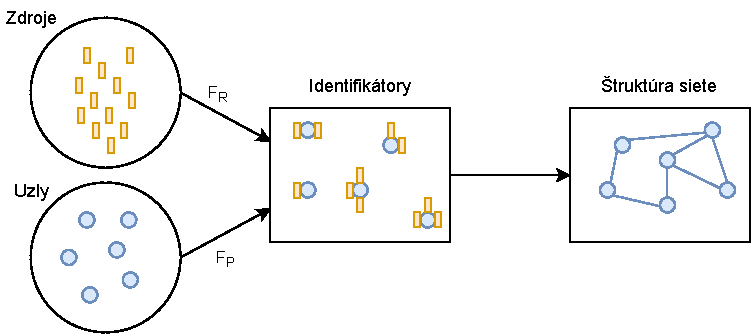
\includegraphics[width=\textwidth]{obrazky-figures/p2p-ref-model.pdf}
	\caption{Referenčný model peer-to-peer siete.~\cite{p2pEssence}}
	\label{img:p2p-ref-model}
\end{figure}

\section{Kryptografia v~BC}\label{sec:crypto}
Pre pochopenie technológie BC je potrebná základná znalosť modernej kryptografie. V~tejto sekcii je popísaný kryptografická hashovacia funkcia (pozri~\ref{subsec:hash}) a jej využitie na tvorbu dátových štruktúr zabezpečených proti modifikácii obsahu (viď sekcia~\ref{subsec:hash-pointer}). Ďalej je vysvetlený koncept asymetrickej kryptografie a digitálneho podpisu (viď sekcia~\ref{subsec:sign}). Tieto kryptografické primitíva sú základom na ktorom stojí nemennosť, auditovateľnosť a anonymita BC.

\subsection{Hashovacia funkcia}\label{subsec:hash}
Hashovacia funkcia je taká funkcia $h$, ktorá má ako parameter $x$ reťazec bitov ľubovolnej dĺžky a vracia reťazec $y$ s~konštantnou dĺžkou(viď rovnica~\ref{eq:hash}). Reťazec $y$ voláme hash. Hashovacia funkcia vracia pre konkrétny vstup vždy rovnaký hash.

\begin{equation} \label{eq:hash}
	h(x) = y
\end{equation}
Kryptografická hashovacia funkcia, alebo tiež jednocestná funkcia (anglicky \textit{one way function}), je taká hashovacia funkcia pre ktorú platia nasledujíce tri vlastnosti:
\begin{enumerate}
	\item Pre daný hash $x$ je výpočetne nezvládnuteľné nájsť správu takú, že $ h(x) = y $. Anglicky voláme túto vlastnosť \textit{first preimage resistant}.
	\item Pre danú správu je výpočetne nezvládnuteľné nájsť inú správu s~rovnakým hashom. Anglicky voláme túto vlastnosť \textit{second preimage resistant}.
	\item Pre ľubovoľnú správu je výpočetne nezvládnuteľné nájsť inú správu s~rovnakým hashom. Anglicky voláme túto vlastnosť \textit{collision resistant}.
\end{enumerate}

Hashovacie funkcie majú v~oblasti počítačovej bezpečnosti dôležité využitie:
\begin{itemize}
	\item Bezpečné ukladanie hesiel: Digitálna služba neukladá v~databáze heslo, ale len jeho hash. Pri ukradnutí databázy nedochádza k~odhalenie hesiel užívateľov.
	\item Integrita dát: Hashovacia funkcia môže byť použitá na ochranu integrity ľubovoľných dát. Ak spočítate hash veľkého súboru a bezpečne ho uložíte tak ste schopný detekovať, že niekto tento súbor zmenil.
	\item Digitálny podpis: Hashovacia funkcia je kryptografické primitívum potrebné pre vytvorenie digitálneho podpisu.
\end{itemize}
Existuje množstvo hashovacích funkcií. Medzi veľmi známe a používané patrí napríklad MD5 (128 bitový výstup), SHA256 (256 bitový výstup), SHA512 (512 bitový výstup).~\cite{cryptoHandbook, nigelSmartCrypto}

\subsection{Hash ukazovateľ}\label{subsec:hash-pointer}
Hash ukazovateľ (anglicky \textit{hash pointer}) je primitívom pre tvorbu dátových štruktúr s~kryptografickým zabezpečením proti manipulácia s~obsahom (anglicky \textit{tamper-evident}). Hash ukazovateľ funguje ako klasický ukazovateľ v~zozname či strome. Navyše však neumožňuje meniť už pridané prvky. Jediná povolená operácia je pridanie ďalšieho prvku do dátovej štruktúry. 

Obrázok~\ref{img:hash-pointer} demonštruje rozdiel medzi zoznamom vytvoreným pomocou klasických ukazovateľov a pomocou hash ukazovateľov. Bežný zoznam umožňuje pozmeniť ľubovoľný už existujúci prvok nezávisle na zvyšku zoznamu. Naopak, hash pointer referencuje pomocou samotného dátového obsahu. Ak by sme zmenili dátový obsah prvku B, tak by sa narušila referencia v~predchádzajúcom prvku.
~\cite{horizenAcademy, narayanan2016bitcoin}


\begin{figure}[bt]
	\centering
	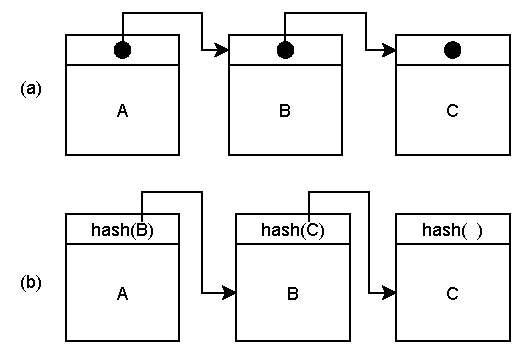
\includegraphics[width=.6\textwidth]{obrazky-figures/hash-pointer}
	\caption{(a) Zoznam pomocou ukazovateľov \medspace (b) Zoznam pomocou hash ukazovateľov}
	\label{img:hash-pointer}
\end{figure}

\subsection{Digitálny podpis}\label{subsec:sign}
Digitálny podpis (anglicky \textit{digital signature}) je kryptografický koncept používaný na autentifikáciu, autorizáciu a nepopierateľnosť. Digitálny podpis jednoznačne prepojí určitú entitu s~informáciu. V~technológii blockchain slúži digitálny podpis na určenie vlastníctva zdrojov, ktoré blockchain uchováva.~\cite{cryptoHandbook, satoshiBitcoin}

Moderná kryptografia používa pre zaistenie dôvernosti šifrovanie pomocou tajného kľúča. Pre zašifrovanie a dešifrovanie tajnej správy je potrebná znalosť tajného kľúča. Tento mechanizmus  zaisťuje dôvernosť avšak nezaisťuje nepopierateľnosť pretože obe komunikujúce strany poznajú tajný kľúč a teda nie je možné právne dokázať kto správu napísal. Na zaistenie nepopierateľnosti sa používa asymetrické šifrovanie, ktoré používa dvojicu kľúčov:
\begin{itemize}
	\item \textbf{Privátny kľúč} je tajný a pozná ho len odosielateľ správy. Odosielateľ používa tento kľúč na zašifrovanie správy.
	\item \textbf{Verejný kľúč} je dostupný komukoľvek. Ktokoľvek s~týmto kľúčom dokáže dešifrovať správu.
\end{itemize}
Tieto dva kľúče tvoria dvojicu prepojenú matematickým spôsobom. Zo znalosti verejného kľúča je výpočetne nezvládnuteľné zistiť privátny kľúč. Zašifrovaná správa nie je dôverná pretože ktokoľvek môže použiť verejný kľúč na jej dešifrovanie. Avšak zašifrovaná správa je nepopierateľne napísaná vlastníkom privátneho kľúča. 

Tento koncept je základom digitálneho podpisu. Ak chceme nepopierateľne dokázať, že nejaký dátový obsah (napríklad pdf dokument) sme vytvorili mi, tak vypočítame jeho hash (viď sekcia~\ref{subsec:hash}) a zašifrujeme ho naším privátnym kľúčom. Zašifrovaný hash priložíme k~dokumentu. Príjemca dokumentu si následne pomocou verejného kľúča dešifruje hash priložený k~správe a porovná si ho s~tým ktorý vypočítal sám z~danej správy. Ak sú hashe rovnaké tak nikto správu nezmenil a dokument je jednoznačne vytvorený vlastníkom tajného kľúča. Najznámejšie algoritmy na digitálny podpis sú RSA, DSA, ECDSA.~\cite{cryptoHandbook}

\subsection{Prahový digitálny podpis}\label{subsec:threshold-sig}
Prahový digitálny podpis (anglicky \textit{threshold signatures}) je špeciálna schéma digitálneho podpisu. V~tejto schéme je $n$ účastníkov a každý vlastní časť privátneho kľúča. Každý účastník môže použiť svoju časť tajného kľúča na čiastočné podpísanie správy $M$. Kompletný podpis môže byť zostrojený ak aspoň $t$ účastníkov poskytlo svoju časť podpisu. Potom hovoríme o~$t$-z-$n$ prahovom podpise. Takýto koncept sa dá využiť pri kryptografickom hlasovaní.~\cite{blsSignature}


\section{Dátová štruktúra blockchain}\label{sec:data-struct-blockchain}
Blockchain je dátová štruktúra podobná zoznamu (anglicky \textit{linked list}). Blockchain organizuje dáta do podmnožín, ktoré sa volajú bloky. Blok je podobný uzlu v~zozname. Každý blok obsahuje referenciu na ďalší blok. Rozdiel medzi zoznamom a blockchainom je v~tom, že referencia blockchainu je zabezpečená proti manipulácia (anglicky \textit{tamper-evident}) pomocou modernej kryptografie. Bežný zoznam používa referenciu pomocou ukazovateľov (anglicky \textit{pointers}), ktoré môže ktokoľvek a kedykoľvek pozmeniť bez toho aby pozmenil dátový obsah. Naopak, blockchain vôbec neumožňuje meniť už pridané bloky. Jediná povolená operácia je pridanie ďalšieho bloku na koniec blockchainu.~\cite{horizenAcademy}

Každý blok obsahuje dáta, ktoré sú typicky vo forme transakcií. Kryptograficky bezpečný blockchain by mohol fungovať aj tak, že v~každom bloku bude uložená práve jedna transakcia. Z~dôvodu optimalizácie je ale v~jednom bloku uložené množstvo transakcií. Vďaka tejto optimalizácii nemusí celá sieť vytvárať konsenzus po každej transakcii. Samotné transakcie v~rámci jedného bloku sú ukladané v~ďalšej dátovej štruktúre, ktorá taktiež používa kryptografické hashovanie (viď sekcia~\ref{subsec:merkle-tree}).~\cite{narayanan2016bitcoin}

\subsection{Blok}\label{subsec:block}

Blok sa skladá z~hlavičky a tela. Telo bloku obsahuje dáta a hlavička obsahuje metadáta. Dáta v~tele bloku sú uložené vo forme transakcií. Transakcie sú popísané v~sekcii~\ref{subsec:transaction}. Počet transakcií v~bloku je typicky obmedzený maximálnou veľkosťou bloku.
Hlavička bloku obsahuje metadáta o~bloku, kde najdôležitejšie a najbežnejšie sú nasledujúce~\cite{zhengBlockchainOverview}:
\begin{itemize}
	\item Hash všetkých transakcií.
	\item Časové razítko vytvorenia bloku.
	\item Hash ukazovateľ na predošlý blok v~blockchaine.
\end{itemize} 

\subsection{Transakcia}\label{subsec:transaction}
Transakcia je elementárna dátová jednotka na ukladanie digitálnych informácií v~blockchaine. Bitcoin, prvý blockchain, použil transakciu na manipuláciu s~elektronickými financiami. Takáto transakcia sa skladá z~troch častí~\cite{narayanan2016bitcoin}:
\begin{itemize}
	\item \textbf{Množina vstupov}: Každý vstup má uložený hash predošlej transakcie s~ktorej vychádza. Ďalej definuje, ktoré výstupy s~predošlej transakcie si nárokuje. Nakoniec obsahuje digitálny podpis, ktorý autorizuje tvorcu transakcie.
	\item \textbf{Množina výstupov}: Každý výstup má hodnotu, ktorá je uchovávaná v~blockchaine (typicky minca nejakej kryptomeny). Suma hodnôt všetkých výstup transakcie musí byť menšia alebo rovná sume všetkých vstupov transakcie. Ak je menšia, tak tento rozdiel je použitý ako odmena pre toho, kto publikoval tento blok blockchainu.
	\item \textbf{Hlavička}: Obsahuje hash transakcie, ktorý je používaný ako unikátny identifikátor pomocou, ktorého sa na transakciu odkazujeme.
\end{itemize}


\subsection{Markle tree}~\label{subsec:merkle-tree}
Binárny hashovací strom alebo tiež Merkle strom (anglicky \textit{Merkle tree})~\cite{merkleTreeBosamia} je dátová štruktúra podobná binárnemu stromu, ktorá slúži na efektívne a rýchle vypočítanie hashu veľkého množstva dát. Blockchain používa tento strom na časovo efektívny výpočet hashu všetkých transakcií. Takto vypočítaný hash je uložený v~hlavičke bloku.

Merkle strom je vyvážený binárny strom, kde listové uzly obsahujú jednotlivé transakcie uložené v~danom bloku blockchainu. Každý nelistový uzol stromu obsahuje hash vypočítaný z~jeho potomkov. Koreňový uzol teda obsahuje hash celého stromu a teda aj všetkých transakcií. Pridanie, odobranie, zmena obsahu, alebo zmena poradia transakcií bude teda viesť k~zmene koreňového hashu. Konštrukcia stromu, inak povedané výpočet hashu všetkých transakcií, prebieha následovne:
\begin{enumerate}
	\item Všetky transakcie sú uložené do listovej úrovne stromu. Ak je počet transakcií nepárny tak, je posledná vložená dvakrát.
	\item Nad každým listovým uzlom je vypočítaný hash.
	\item Každý nelistový uzol skonkatenuje hash ľavého a pravého syna, vypočíta nad nimi hash a uloží si ho. 
\end{enumerate}
Konštrukcia takéhoto stromu pre $n$ transakcií má časovú zložitosť $O(log(n))$. Takýto spôsob výpočtu hashu je teda veľmi efektívny pre veľké množstvo transakcií (blok v~blockchaine bežne obsahuje stovky transakcií).

Merkle strom umožňuje efektívne šetriť pamäťové nároky blockchainu. Do blockchainu sú neustále pridávané nové bloky, ktoré obsahujú aj rovnaké staré transakcie. Ak už sú transakcie zaznamenané v~dostatočne veľkom množstve blokov tak sú z~hľadiska bezpečnosti nemenné. V~nových blokoch ich už preto nie je potrebné ukladať. Nový blok si preto uloží len hashe starých vetiev stromu, ale ich obsah už nepotrebuje. Takto je zachovaná integrita hashu všetkých transakcií.~\cite{satoshiBitcoin}


\chapter{Konsenzus}\label{chap:consenzus}

Konsenzus v~BC zabezpečuje, že skupina uzlov (peerov) sa  zhodne na rovnakom stave BC. Tradične je táto vlastnosť zabezpečená centrálnou autoritou s~ktorou musia byť všetky uzly spojené. Avšak BC je decentralizovaný a teda toto riešenie nie je možné. Konsenzus v~decentralizovanej sieti BC je zabezpečený pomocou protokolu, ktorý sa snaží nájsť kompromis medzi nasledujúcimi troma vlastnosťami (anglicky \textit{CAP theorem})~\cite{gilbertCAP, zhangConsensus, leporeConsensus}:
\begin{itemize}
	\item Konzistentnosť (\textit{Consistency}): Všetci uživatelia majú rovnaký stav BC (rovnaké dáta).
	\item Dostupnosť (\textit{Availability}): Pre každú požiadavku na dáta musí byť poskytnutá odpoveď v~konečnom čase. Odpoveďou môže byť aj neúspech.
	\item Odolnosť voči prerušeniu (\textit{Partial tolerance}): Sieť funguje aj v~prípade, že v~nej vznikajú chyby (výpadky uzlov, škodlivé správanie časti uzlov).
\end{itemize}
CAP theorem~\cite{gilbertCAP} deklaruje, že z~týchto troch vlastností je súčasne možné dosiahnuť maximálne dve.

Technológia BC požaduje decentralizovanú distribuovanú sieť. Z~vlastností takejto siete je zrejmé, že BC musí nevyhnutne riešiť problém odolnosť voči prerušeniu. Zo zvyšných dvoch vlastností sa môže zvoliť dostupnosť pred konzistenciou (napríklad Bitcoin). Bitcoin zaisťuje konzistenciu až dodatočne (anglicky \textit{eventual consistancy}) pomocou procesu ťažby blokov a určenia najdlhšieho reťazca. Druhou možnosťou je zvoliť konzistenciu pred dostupnosťou. Táto skupina BC protokolov je založená na hlasovaní pomocou PBFT protokolu (viď~\ref{subsec:pos-pbft}) na zaručenie silnej konzistencie.~\cite{capViswanath}

\section{Typy konsenzus protokolov}
Existujú tri najbežnejšie techniky, ktoré sa používajú pre ustavenie konsenzu~\cite{zhangConsensus, homoliakBlockchain}:
\begin{itemize}
	\item \textbf{Lotéria}: Takéto protokoly náhodne zvolia uzol, ktorý vyprodukuje nový blok. Výhodou tohoto prístupu je jeho jednoduchosť keďže takýto proces nevyžaduje žiadnu interaktívnu komunikáciu. Nevýhodou tohoto prístupu je, že pripúšťa možnosť voľby viacerých uzlov súčasne. V~takom prípade sa reťazec rozvetví (anglicky \textit{fork}) a je potrebné určiť ktorá vetva je správna. Typicky sa za správnu vetvu volí tá najdlhšia. Avšak takéto správanie oslabuje konzistentnosť BC. Transakcie v~posledných blokoch môžu byť potenciálne zahodené pretože nejde o~správnu vetvu. Preto sa za konzistentné transakcie považujú až tie ktoré sú prekryté väčším množstvom nových blokov.
	\item \textbf{Hlasovanie}: Protokoly založené na hlasovaní dosahujú dohodu pomocou hlasovania všetkých zapojených uzlov. Môžeme použiť napríklad protokol Byzantskej chyby (anglicky \textit{Byzant fault tolerance}), ktorý vyžaduje majoritu hlasov k~uzavretiu konsenzu (typicky $\frac{2}{3}$). Výhodou je veľmi malá pravdepodobnosť vzniku vetiev reťazca. Na druhej strane, takéto protokoly majú nižšiu priepustnosť, ktorá klesá z~narastajúcim počtom uzlov.
	\item \textbf{Kombinovaný prístup}: Tieto protokoly sa snažia kombinovať prístup lotérie a hlasovania s~cieľom dosiahnuť výhody oboch prístupov. Napríklad je možné rozdeliť počet uzlov podieľajúcich sa na hlasovaní pomocou lotérie, čím sa zvýši priepustnosť.
\end{itemize}

Dnes sa hovorí najmä o~dvoch rodinách konsenzus protokolov. Prvou a najbežnejšou rodinou je \textit{Proof-of-Work}. Tento konsenzus mechanizmus je založený na princípe lotérie. Detailnejšie je popísaný v~sekcii~\ref{sec:pow}.

Táto práca sa však zaoberá predovšetkým konsenzus mechanizmom, ktorý sa všeobecne nazýva \textit{Proof-of-Stake}. Táto rodina konsenzus protokolov je založená na hlasovaní. V~poslednej dobe sa ponúka ako vhodná alternatíva k~Proof-of-Work. Tento mechanizmus je detailnejšie popísaný v~sekcii~\ref{sec:pos}

\section{Proof-of-Work}\label{sec:pow}
Dôkaz prácou, anglicky \textit{Proof-of-Work} (ďalej PoW), je najbežnejšia stratégia konsenzus protokolu. Ak chce uzol publikovať nový blok, musí investovať svoj výpočtový výkon do riešenia netriviálneho kryptografického problému. Uzol, ktorý ako prvý vyrieši tento problém má najväčšiu pravdepodobnosť, že bude jeho blok pridaný do reťazca. Samozrejme, je tu možnosť, že problém vyrieši súčasne viacero uzlov. Konečná voľba je teda náhodná. PoW teda umožňuje, aj keď s~oveľa menšou pravdepodobnosťou, že sa reťazec rozvetví. Bezpečnosť takéhoto konsenzu spočíva v~tom, že majorita výpočtového výkonu siete (51\,\%) je vlastnená poctivými uzlami.

PoW konsenzus využíva dva typy uzlov. Prvý typ uzla je miner, ktorý vytvára nové bloky tak ako je popísané v~sekcii~\ref{sec:mining}. Druhý typ uzla je bežný vlastník zdrojov v~danom BC, ktorý môže vytvárať transakcie a distribuovať ich do siete. Druhý typ uzla teda nehrá žiadnu rolu v~ustanovovaní konsenzu.~\cite{leporeConsensus}

\subsection{Ťažba blokov}\label{sec:mining}

Ťažba (anglicky \textit{mining})~\cite{narayanan2016bitcoin} bloku je proces pridania nové bloku na koniec blockchainu. Ťažba bloku zahŕňa validáciu transakcií a blokov. Preto je ťažba kritická pre správne a bezpečné fungovanie blockchainu. Každý uzol siete, ktorý ťaží nové bloky sa nazýva anglickým slovom \textit{miner}. Tieto uzly umožňujú rozširovanie blockchainu. Aby takéto uzly existovali, musia byť motivované. Miner dostane za každý vyťažený blok ako odmenu zdroje uložené v~blockchaine.

Ťažba všeobecne pozostáva z~nasledujúcich krokov:
\begin{enumerate}
	\item Miner prijíma požiadavky na transakcie z~peer-to-peer siete. Každú transakciu si validuje pomocou kryptografie popísanej v~sekcii~\ref{sec:crypto}. Miner musí taktiež udržiavať aktuálny stav blockchainu. Je potrebné sledovať či nevznikli nové bloky a udržiavať si validný blockchain.
	\item Ak miner vlastní validnú a aktuálnu kópiu blockchainu a má dostatok transakcií, môže začať vytvárať nový blok. Do nového bloku vloží transakcie, ktoré prijal a boli validné. Následne investuje svoj výpočtový výkon do vyriešenia kryptografického problému (podrobnejšie popísané v~sekcii~\ref{subsec:bitcoin}). Ak úlohu vyrieši tak môže zostrojiť nový validný blok.
	\item Novo vytvorený blok je potrebné distribuovať do siete. Ak väčšina siete blok získa a akceptuje, tak bol pridaný do blockchainu.
	\item Ak sa podarilo úspešne blok pridať do blockchainu tak miner získava odmenu. Odmena za vyťažený blok je konštantná čiastka zdrojov poskytovaných daným blockchainom. Napríklad Bitcon poskytuje v~roku 2021 ako odmenu 6,25 bitcoinov čo je približne 300 dolárov~\footnote{\url{https://www.investopedia.com/tech/how-does-bitcoin-mining-work/}}. Avšak táto odmena môže byť zvýšená o~poplatky, ktoré sú v~transakciách. Ak teda chcete aby sa vaša transakcia dostala do blockchainu čo najrýchlejšie, poskytnete vyššiu odmenu v~podobe poplatku za transakciu. Miner bude potom viac motivovaný pridať práve túto transakciu do bloku.
\end{enumerate}

\subsection{Bitcoin}\label{subsec:bitcoin}
Bitcoin je najznámejší BC protokol, ktorý používa PoW konsenzus. Samotný kryptografický problém, ktorý užívatelia tejto siete riešia spočíva v~počítaní hashu (viď~\ref{subsec:hash}) z~hlavičky nového bloku (viď~\ref{subsec:block}). Hlavička obsahuje atribút nonce, ktorý môže miner ľubovolne nastaviť. Zmenou tohoto atribútu môže miner získať iný hash hlavičky bloku. Konsenzus vyžaduje aby výsledná hash hodnota bola menšia rovná určitej zvolenej hodnote. Miner môže túto podmienku dosiahnuť len tak, že bude inkrementovať hodnotu atribútu nonce až dokedy túto podmienku nesplní. Táto úloha sa teda dá riešiť len pomocou metódy útok hrubou silou (anglicky \textit{brute force}). Miner môže svoju šancu na úspech zvýšiť len tým, že poskytne väčší výpočtový výkon do jej riešenia. Na druhej strane, ostatné uzly môžu overiť, že jeho riešenie je správne veľmi rýchlo a efektívne.~\cite{zhengBlockchainOverview}

\subsection{Vlastnosti}
PoW je overený konsenzus protokol, ktorý funguje a používa sa v~blockchainoch ako je Bitcoin~\cite{satoshiBitcoin} alebo Ethereum~\footnote{\url{https://ethereum.org/en/whitepaper/}}. Tento protokol má však jeden dlhodobý problém a to je spotreba energie. Uzly ktoré riešia kryptografický problém pre nové bloky spotrebujú veľké množstvo energie čo má nepriaznivý dopad na životné prostredie. Niektoré zdroje~\footnote{\url{https://www.businessinsider.com/bitcoin-mining-electricity-usage-more-than-google-2021-9}} napríklad hovoria, že v~roku 2021 pokrýva ťažba Bitcoinu 0,5\,\% celkovej spotreby elektrickej energie na svete. Pre porovnanie, ide o~sedemkrát väčšiu spotrebu energie ako má celá spoločnosť Google.~\cite{leporeConsensus}

Druhou veľkou nevýhodou Bitcoinu je jeho slabá priepustnosť transakcií (\textit{TPS - transaction per second}). TPS je metrika kľúčová napríklad v~oblasti kryptomien. Pre porovnanie, centralizovaný platobný systém VISA~\footnote{\url{https://towardsdatascience.com/the-blockchain-scalability-problem-the-race-for-visa-like-transaction-speed-5cce48f9d44}} má TPS približne 1\,500 zatiaľ čo Bitcoin približne~5.

\section{Proof-of-Stake}\label{sec:pos}

Dôkaz podielom na vlastníctve, anglicky \textit{Proof-of-Stake} (ďalej PoS), je založený na technike lotérie, kde pravdepodobnosť výhry rastie s~množstvom už vlastnených zdrojov. Základnou myšlienkou, je že vlastník veľkého množstva zdrojov v~danom BC je veľmi nepravdepodobným útočníkom pretože svoje zdroje nechce ohroziť. Uzly sa teda musia preukázať vlastníctvom zdrojov v~danom BC ak chcú publikovať nový blok. Pravdepodobnosť výberu uzlu rastie s~množstvom zdrojov, ktoré v~sieti vlastní.~\cite{homoliakBlockchain, nguyenPos}

\subsection{Vlastnosti}

Veľkou výhodou PoS oproti PoW je, že nevyžaduje také veľké množstvo energie. Uzly už nemusia súťažiť v~riešení výpočtovo náročných úloh. Ďalšou veľkou výhodou je rýchlosť. PoS konsenzus umožňuje rádovo vyššie TPS, ktoré je v~prípade PoW značne limitované.~\cite{leporeConsensus, nguyenPos}

PoS konsenzus však prináša aj viaceré problémy. Najväčším problémom je bezpečnosť. PoS prinieslo nové typy útokov, ktoré pri PoW nevznikali. Tieto útoky sú podrobnejšie popísané v~sekcii~\ref{sec:pos-attacks}. Bežným problémom väčšiny PoS protokolov je, že nedefinujú teoretický základ a formálne definovanú bezpečnosť. Existujú teda rôzne riešenia na tieto útoky avšak neexistuje formálny bezpečnostný model, ktorý by dokazoval, že tieto útoky sú zabezpečené.

Ďalším problémom je model motivácie. PoS konsenzus podporuje validné správanie odmeňovaním v~podobe zdrojov. Naopak, škodlivé chovanie je trestané ich odoberaním. Problémom tohoto mechanizmu je jeho nejednoznačná definícia. Väčšina protokolov neobsahuje formálnu analýzu ich modelu motivácie.~\cite{nguyenPos}

\section{Proof-of-Authority}

PoA~\cite{Angelis2018PBFTVP} je rodina konsenzus protokolov založená na algoritmoch BFT (\textit{Byzantian Fault Tolerance}). PoA predpokladá, že v~sieti je $N$ dôveryhodných uzlov. Tieto uzly (autority) sú jednoznačne identifikované  a majorita autorít je poctivá (konkrétne $N/2 + 1$). Veľmi rozšírený PoA protokol je PBFT popísaný v~sekcii~\ref{subsec:pos-pbft}.

\subsection{Practical Byzantine Fault Tolerance}\label{subsec:pos-pbft}

\textit{Practical Byzantine Fault Tolerance}~\cite{pbftCastro} (ďalej len PBFT) je protokol na uznesenie konsenzu v~distribuovanej sieti pomocou hlasovania. Tento protokol patrí do rodiny proof-of-authority. Avšak je často používaný aj v~rámci PoS konsenzu. PoS protokoly často vyžadujú interné hlasovanie ktoré sa často rieši práve pomocou PBFT, kde dôveryhodnosť uzlov je zabezpečená vlastníctvom zdrojov (PoS). PBFT funguje pod podmienkou, že v~sieti je maximálne $\frac{1}{3}$ nepoctivých uzlov. Na komunikáciu v~sieti sa používa všesmerové vysielanie (anglicky \textit{broadcast}). Na zabezpečenie sa požíva kryptografia s~digitálnym podpisom (viď sekcia~\ref{subsec:sign}). Jednotlivé uzly môžu posielať požiadavky do siete (vtedy hovoríme o~tomto uzle ako o~klientovi). Protokol definuje jeden uzol v~sieti ako vodcu a ostatné uzly ako validátorov. Vodca hlasovania sa pravidelne mení podľa dohodnutého rozvrhu.
Hlasovanie protokolu prebieha v~štyroch fázach:
\begin{enumerate}
	\item \textit{Request}: Klient zašle vodcovi požiadavku na uznesenie konsenzu v~sieti.
	\item \textit{Pre-prepare}: Vodca rozošle požiadavku všetkým validátorom.
	\item \textit{Prepare}: Validátori overia požiadavku, ak súhlasia, tak pošlú svoj hlas všetkým v~sieti. Zároveň, každý uzol siete (validátori aj vodca) sledujú a overujú hlasy, ktoré prijali. Ak uzol zaznamenal viac ako $\frac{2}{3}$ hlasov tak zašle potvrdenie všetkým uzlom v~sieti. 
	\item \textit{Commit}: Každý uzol počíta potvrdenia od všetkých ostatných uzlov v~sieti. Ak získa viac ako~$\frac{1}{3}$ potvrdení, tak pošle potvrdenie klientovi, ktorý pôvodne inicializoval požiadavku na konsenzus. Klient vie, že jeho požiadavka bola prijatá sieťou, ak prijme viac ako $\frac{1}{3}$ potvrdení.
\end{enumerate}
Obrázok~\ref{img:pbft} demonštruje tento protokol. \textbf{C} je klient, uzol 0 je vodca a uzly 1 až 3 sú validátori. Môžeme vidieť, že sieť funguje aj keď uzol 3 nereaguje na komunikáciu.
\begin{figure}[bt]
	\centering
	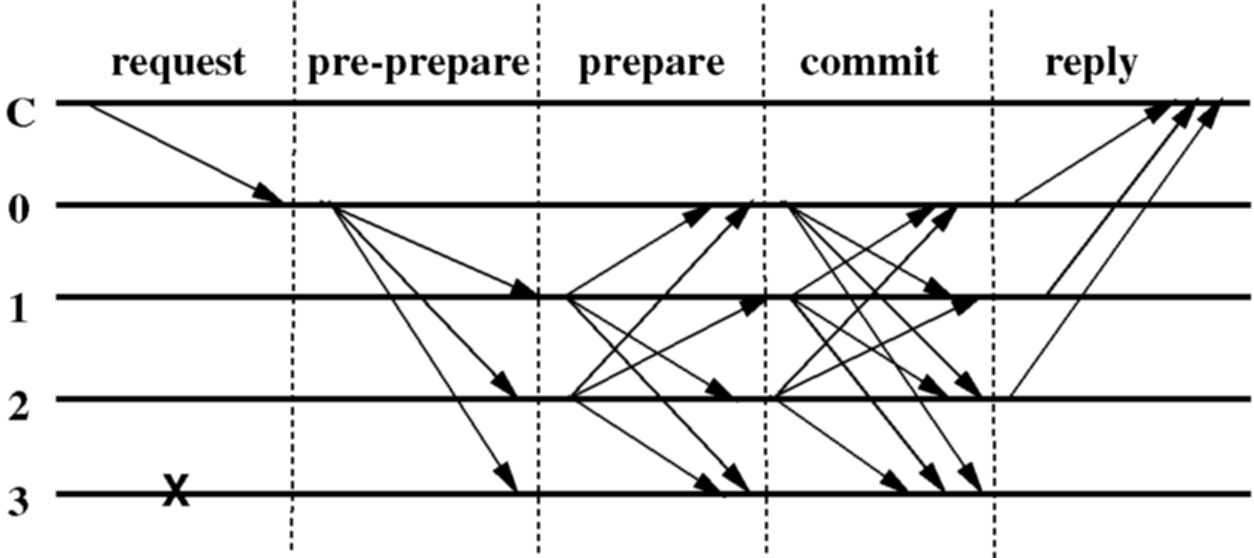
\includegraphics[width=.7\textwidth]{obrazky-figures/pbft}
	\caption{Priebeh hlasovania v~PBFT (prevzaté z~\cite{pbftCastro}).}
	\label{img:pbft}
\end{figure}

\section{Všeobecné útoky na konsenzus}
Nasledujúca sekcia vysvetľuje najbežnejšie typy útokov na bezpečnosť konsenzus protokolov. Ide o~útoky, ktoré sú aplikovateľné na všetky rodiny konsenzus protokolov. Ďalej popísané útoky vychádzajú z~nasledujúcej práce~\cite{homoliakBlockchain}. 

\subsection{Ovládnutie konsenzu útočníkmi}
Tento útok naruší decentralizovanosť siete tým, že útočníci dokážu utvoriť konsenzus aj bez poctivých uzlov. V~takom prípade sa stáva sieť centralizovaná, kde centrálnou autoritou sú práve útočníci. Príkladom takéhoto útoku pre PoW a PoS konsenzus je ovládnutie 51\,\% siete. V~prípade protokolov Byzantskej chyby dokáže $\frac{1}{3}$ uzlov spôsobiť, že bude protokol narušený alebo dokonca zastavený.

\subsection{Porušenie synchronného doručovania}

Ak útočník dokáže narušiť synchrónne doručovanie správ v~protokole, ktorý synchronizáciu predpokladá tak takýto protokol prestane fungovať. Tento útok už nie je možné urobiť na protokole, ktorý umožňuje asynchronnú komunikáciu. Tento útok je možné vykonať napríklad pre protokoly Byzantskej chyby.

\subsection{Útok na časovú synchronizáciu}
Decentralizovaná sieť BC potrebuje časovú synchronizáciu medzi uzlami. Pri vytvorení nového bloku sa do jeho hlavičky zvyčajne vkladá aj časové razítko (anglicky \textit{timestamp}). Jednotlivé uzly v~sieti majú vlastný čas, ktorý typicky vypočítavajú ako medián všetkých časov získaných od ostatných. Tvorca nového bloku potom vloží do hlavičky práve takto vypočítaný čas. Ostatné uzly v~sieti budú pri distribúcii bloku overovať, že čas je dostatočne aktuálny aby bol akceptovaný. Ak útočník disponuje veľkým množstvom uzlov v~sieti, tak môže narušiť synchronizáciu času, ktorý bloky získavajú mediánom. Tento útok následne spomaľuje sieť pretože bloky distribuujú bloky s~časovou značkou, ktorá už nebude akceptovaná.

\subsection{Zdvojnásobenie výdavkov}

Zdvojnásobenie výdavkov (anglicky \textit{double spending}) je útok, ktorý vzniká vytvorením dvoch alebo viac konfliktných blokov. Tieto bloky vytvárajú tzv. vetvy (anglicky \textit{forks}). S~tohoto dôvodu môžu byť niektoré krypto mince dočasne minuté v~oboch konfliktných blokoch. Neskôr je síce len jeden z~nich validný pretože druhá vetva bude zahodená. Avšak tento útok spomaľuje konzistentnosť blockchainu. Tento útok už bol popísaný aj v~sekcii~\ref{subsec:bc-usage}.

\subsection{Útok na podskupiny uzlov}\label{subsec:shard-attack}

Niektoré konsenzus protokoly rozdeľujú celú sieť na podskupiny uzlov (anglicky \textit{shards}). Sharding zvyšuje škálovateľnosť a priepustnosť siete pretože uzly validujú transakcie len v~rámci svojej podskupiny. Na druhej strane, tento prístup môže viesť k~zníženie bezpečnosti. Množstvo spolupracujúcich uzlov v~jednej takejto podskupine je oveľa menší než v~celej sieti. Pre útočníka môže byť preto jednoduchšie ovládnuť takúto podskupinu ako celú sieť.

%\subsection{Útok posledného objaviteľa}\label{subsec:lst-re-attack}
%
%last-revealer attack~\cite{lastRevealerAttack}

\section{Útoky na Proof-of-Stake}\label{sec:pos-attacks}
V~tejto sekcii sa pozrieme na útoky špecifické pre PoS konsenzus protokoly. Vymenované útoky sú definované v~tejto práci~\cite{homoliakBlockchain}.

\subsection{Vetvenie bez rizika straty zdrojov}
Generovanie blokov v~PoS nestojí žiadnu energiu v~podobe výpočtového výkonu. Uzly preto môžu generovať viacero konfliktných uzlov súčasne a tým zvyšovať pravdepodobnosť, že bude práve ich uzol pridaný do reťazca. Takéto správanie nepredstavuje pre daný uzol žiaden risk v~podobe straty zdrojov. Problémom tohoto správania je, že vzniká väčšie množstvo vetiev reťazca. Ako dôsledok sa potom zvyšuje čas do konzistentnosti BC.

\subsection{Ovplyvnenie volieb}\label{subsec:grinding-attack}
PoS protokoly často potrebujú aby podielnici hlasovali. Na to používajú hlasovacie protokoly z~rodiny BFT. Ako bolo popísané v~sekcii~\ref{subsec:pos-pbft}, tieto protokoly typicky fungujú tak, že jeden uzol (vodca) vedie voľby a ostatné uzly (validátori) ich overujú a potvrdzujú. Roľa vodcu má rôzne výhody (napríklad niektoré BC odmeňujú vodcu podielom z~poplatkov za vložené transakcie do bloku). Útočník preto môže chcieť ovplyvniť voľbu vodcu v~svoj prospech. Na určenie, ktorý uzol sa stane vodcom sa často používa nejaká forma náhodnosti, ktorá je distribuovane generovaná. Útočník môže ovplyvniť generovanie tejto náhodnosti vo svoj prospech, tak aby sa stal vodcom práve on.

\subsection{Odmietnutie služby lídrovi/výboru}\label{subsec:leader-dos}

Ako už bolo spomenuté v~sekcii~\ref{subsec:grinding-attack}, PoS protokoly často používajú BFT hlasovanie v~ktorom je kľúčová roľa vodcu bez ktorého hlasovanie neprebehne. Niektoré PoS protokoly vytvárajú rozvrh vodcov na dlhšie časové obdobie. Takýto rozvrh je dopredu známi čo zjednodušuje a zrýchľuje celý konsenzus. Na druhej strane, útočníci dopredu vedia, ktorý uzol bude v~konkrétnom čase vodcom. Útočník potom môže v~danom čase vykonať DoS útok na vodcu a znemožniť uzatvárať konsenzus v~BC pomocou hlasovania.

\subsection{Neskoršia korupcia}
Útočník sa snaží získať privátne kľúče uzlov, ktoré mali v~minulosti vplyv na reťazec BC. Útočník ich môže ukradnúť, ale taktiež kúpiť. Tieto uzly môžu byť ochotné predať svoje privátne kľúče pretože tým nič neriskujú. Virtuálne zdroje, ktoré majú vložené do daného BC môžu kedykoľvek vymeniť za reálne peniaze. Ak útočník získa kľúče s~dostatočným podielom zdrojov, tak môže pozmeniť históriu reťazca.

\chapter{Harmony}\label{chap:harmony}

Harmony je BC používajúci PoS konsenzus a \textit{sharding}. Cieľom tohoto protokolu je poskytovať aplikácie, ktoré v~minulosti nebolo možné uskutočňovať na technológii BC z~dôvodu rýchlosti a škálovateľnosti. Harmony je BC, ktorý má poskytovať služby ako decentralizované zmenárne alebo platobný systém rozsahovo porovnateľný s~Visa.

Ak nie je uvedené inak, tak všetky informácie o~protokole Harmony popisované v~tejto kapitole vychádzajú z~oficiálnej dokumentácie publikovanej autormi tohoto protokolu~\cite{harmonyWp, harmonyDoc}. Sekcia~\ref{sec:harmony-cons} popisuje konsenzus protokol. Sekcia~\ref{sec:harmony-shards} vysvetľuje sharding používaný v~tomto protokole a sekcia~\ref{sec:harmony-incenctives} definuje model motivácie. Na záver je v~sekcii~\ref{sec:harmony-analyze} tento protokol analyzovaný z~hľadiska bezpečnosti a výkonnosti.

\section{Konsenzus}\label{sec:harmony-cons}

Konsenzus v~Harmony protokole je založený na algoritme PBFT, ktorý už bol popísaný v~sekcii~\ref{subsec:pos-pbft}. Jeden z~kľúčových problémov PBFT je, že jeho časová zložitosť je $O(n^2)$ pre $n$ uzlov. Táto vlastnosť neumožňuje dobrú škálovatelnosť siete. Avšak Harmony používa úpravu PBFT, ktorá má lineárnu časovú zložitosť vzhľadom k~počtu uzlov v~sieti (viď sekcia~\ref{subsec:fbft}).

\subsection{Protokol FBFT}\label{subsec:fbft}
Pre vygenerovanie nového bloku používa Harmony svoj vlastný protokol FBFT (\textit{Fast Byzantine Fault Tolerance}). FBFT namiesto zasielania hlasov pomocou broadcastu používa prahový digitálny podpis (pozri sekciu~\ref{subsec:threshold-sig}). FBFT konsenzus prebieha následovne:
\begin{enumerate}
	\item Vodca vytvorí blok a rozošle jeho hlavičku aj dátový obsah validátorom pomocou broadcastu.
	\item Validátori príjmu nový blok, overia jeho hlavičku, podpíšu ju svojím digitálnym podpisu a pošlú späť vodcovi. Obsah bloku je zatiaľ ignorovaný.
	\item Keď vodca prijme aspoň $\frac{2}{3}$ podpisov, tak ich agreguje do jediného prahového digitálneho podpisu (viď kryptografický prahový podpis popísaný v~sekcii~\ref{subsec:threshold-sig}). Tento podpis rozošle pomocou broadcastu spolu s~bitmapou indikujúcou validátorov ktorý podpísali.
	\item Každý validátor overí, že prahový podpis obsahuje požadované $\frac{2}{3}$ hlasov. Až v~tejto chvíli validátor overí transakcie v~dátovom obsahu bloku, ktorý bol zasielaný už v~kroku 1. Ak všetko súhlasí, tak podpíše správu s~kroku 3 a pošle ju späť vodcovi.
	\item Vodca čaká na $\frac{2}{3}$ podpisov validátorov s~predošlého kroku (môžu sa líšiť od podpisov z~kroku 3). Opäť ich agreguje do prahového podpisu a spolu s~bitmapou účastníkov rozošle pomocou broadcastu nový blok na potvrdenie všetkým validátorom. 
\end{enumerate}
Obrázok~\ref{img:fbft} demonštruje FBFT protokol pre štyri uzly. Na tomto príklade môžeme vidieť, že celé hlasovanie má lineárnu časovú zložitosť, keďže broadcast vysiela len vodca (na rozdiel od PBFT, kde broadcast vysielajú aj validátori).

Je dôležité podotknúť, že Harmony je PoS konsenzus. Vodca v~skutočnosti nečaká na $\frac{2}{3}$ podpisov, ale len na toľko aby ich vlastníci spoločne vlastnili $\frac{2}{3}$ celkového podielu.

\begin{figure}[bt]
	\centering
	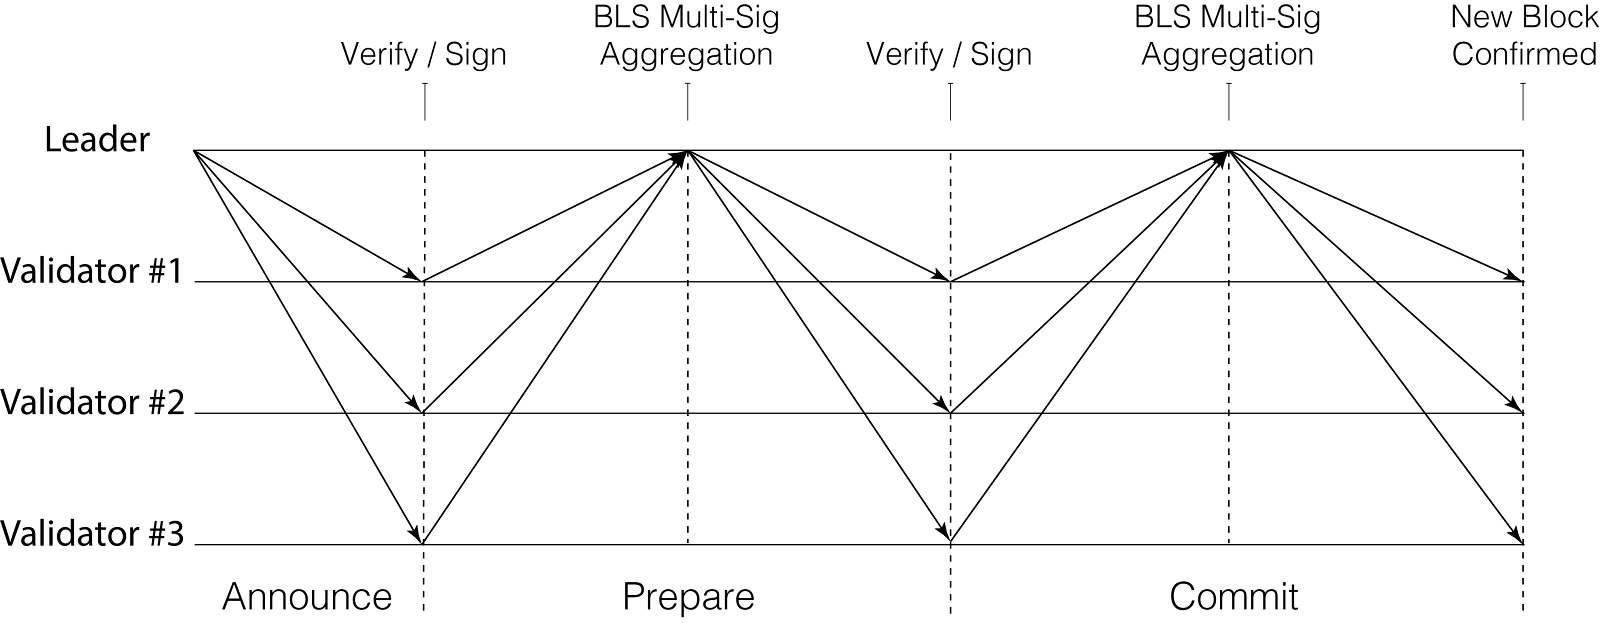
\includegraphics[width=.7\textwidth]{obrazky-figures/harmony-fbft}
	\caption{Priebeh hlasovania v~FBFT (prevzaté z~\cite{harmonyWp}).}
	\label{img:fbft}
\end{figure}

%Uvažujme epocha $e$, každý validátor $v$ má v epoche $e$ podiel $s_v$ a počet jeho hlasovacích lístkov $t_v$. Podiel $s_v$ sa rozdelí na $t_v$ častí, kde každá časť má hodnotu $s_v / t_v$. Všetky časti podielu od všetkých validátorov sa následne zostupne zoradia a vyberie sa z nich prvých $n$. Majiteľ $i$-tého dielu v tejto rade, pre $1 ~\leq i \leq n$, bude vodcom pre $i$-té kolo FBFT v epoche $e+1$.

%Obrázok~\ref{img:harmony-leader} demonštruje protokol na určenie vodcu FBFT protokolu pre jednotlivé bloky v rámci epochy. Všimnime si, že validátori s malým podielom sa vôbec nemusia stať vodcami.

%\begin{figure}[bt]
%	\centering
%	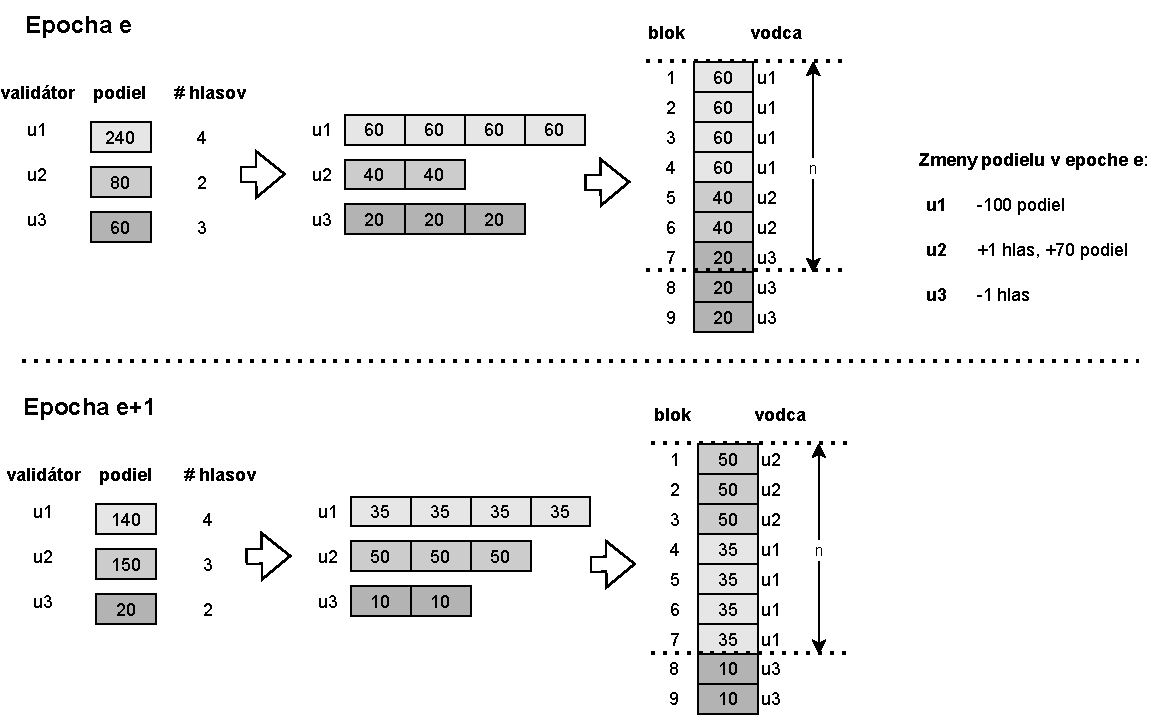
\includegraphics[width=.8\textwidth]{obrazky-figures/harmony-leader}
%	\caption{Vytvorenie rozvrhu vodcov v epoche ktorej dĺžka je 8.~\cite{harmonyDoc}}
%	\label{img:harmony-leader}
%\end{figure}

\section{Sharding}\label{sec:harmony-shards}

Harmony protokol používa \textit{sharding} aby dosiahol lepšiu škálovateľnosť a priepustnosť transakcií. Niektoré zdroje%
\footnote{\url{https://www.investing.com/news/cryptocurrency-news/harmony-one-slow-and-steady-wins-the-race-2609585}} deklarujú, že Harmony má priepustnosť priemerne 2\,000 TPS. Aktuálne používa 4 shardy a autori tvrdia, že pridaním každej ďalšej sa zvýši priepustnosť o~500 TPS. Táto sekcia vysvetľuje celý koncept shardingu v~protokole Harmony.

\subsection{Rozdelenie hlasovacím podielom}\label{subsec:rand-dist}
Ak sa chce uzol stať účastníkom Harmony blockchainu, musí vložiť určité množstvo zdrojov. Tento podiel určuje koľko bude mať hlasovacích lístkov pri validovaní. Tieto hlasovacie lístky sú následne náhodne rozdelené medzi všetky shardy (viď sekcia~\ref{subsec:rnd}) po dobu jednej epochy (viď sekcia~\ref{subsec:epoch}). Tento postup je demonštrovaný na obrázku~\ref{img:harmony-sharding}.

\begin{figure}[bt]
	\centering
	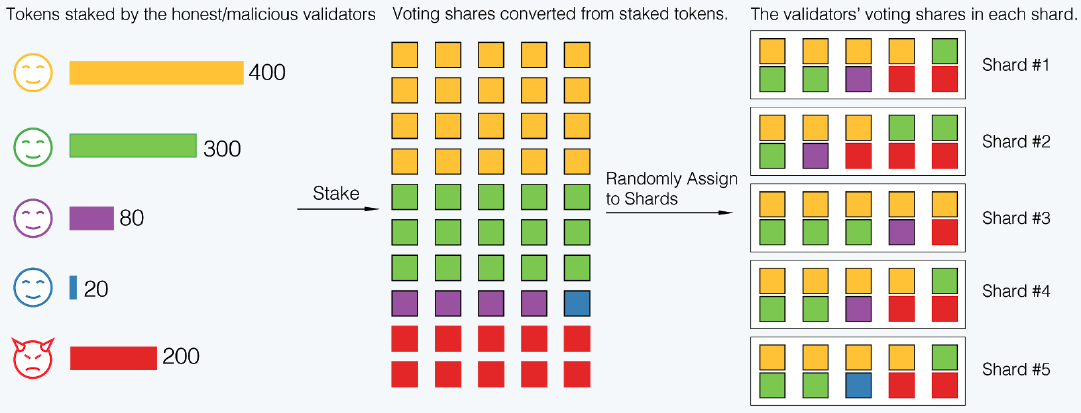
\includegraphics[width=\textwidth]{obrazky-figures/harmony-sharding}
	\caption{Rozdelenie hlasovacieho podielu validátorov medzi všetky shardy (prevzraté z~\cite{harmonyDoc}).}
	\label{img:harmony-sharding}
\end{figure}

\subsection{Epocha}\label{subsec:epoch}
Epocha je časový interval počas, ktorého je štruktúra každého shardu nemenná. Epocha odpovedá času potrebnému na vygenerovanie 32\,768 blokov v~beacon sharde, čo je približne 18,2 hodiny%
\footnote{\url{https://docs.harmony.one/home/network/validators/definitions/epoch-transition}} (koncept beacon shard bude vysvetlený v~sekcii~\ref{subsec:cross-com}). Na začiatku epochy je vygenerované náhodné číslo (pozri sekciu~\ref{subsec:rnd}) na základe ktorého sa vytvorí rozdelenie do shardov. Účastníci, ktorý chcú validovať v~nasledujúcej epoche musia v~aktuálnej vložiť svoj podiel tokenov.


\subsection{Hlasovacie lístky}\label{subsec:harmony-token}
Celkové množstvo hlasovacieho podielul je rozdelené na konštantne veľké tokeny (hlasovacie lístky). Hodnota jedného hlasovacieho lístku $t$ v~epoche $e$ je určená rovnicou~\ref{eq:harmony-vote}, kde $S_{e-1}$ je celkový podiel vložený v~epoche $e-1$, $n$ je počet shardov a $\lambda$ je bezpečnostný parameter. Ak $\lambda > 600$, tak pravdepodobnosť ovládnutia aspoň $\frac{1}{3}$ shardu jedným útočníkom je $0,000\,003$\,\% (dôkaz viď~\cite{harmonyDoc} kapitola 3).

\begin{equation}\label{eq:harmony-vote}
	t = \frac{S_{e-1}}{n . \lambda}
\end{equation}

\subsection{Náhodné rozdelenie hlasovacieho podielu medzi shardy}\label{subsec:rnd}
Harmony rozdeľuje hlasovacie lístky do shardov pomocou náhodnej voľby (anglicky \textit{randomness based sharding}). Na začiatku epochy je vykonaná náhodná permutácia hlasovacieho podielu všetkých podielnikov. Získaná permutácia je rozdelená na $n$ rovnakých častí, kde $n$ je počet shardov. Časť $i$, kde $1 \leq i \leq n$, predstavuje validátorov a ich hlasovací podiel v~sharde $i$. Permutácia je vykonaná na základe náhodného čísla \textit{rnd}, ktoré je generované distribuovane.

Na vygenerovanie \textit{rnd} sa používa algoritmus VRF (\textit{Verifiable Random Function~\cite{algorandGilad}}) a VDF (\textit{Verifiable Delay Function~\cite{vdfBoneh}}). Tento výpočet vykonáva beacon shard (koncept beacon shard bude vysvetlený v~sekcii~\ref{subsec:cross-com}):
\begin{enumerate}
	\item Vodca pošle hash posledného bloku všetkým validátorom.
	\item Každý validátor vypočíta s~prijatého hashu pomocou VRF náhodné číslo, ktoré pošle späť vodcovi.
	\item Keď vodca príjme $\frac{1}{3}$ náhodných čísel, tak nad nimi urobí XOR. Výslednú hodnotu \textit{pRand} vloží do nového bloku pomocou FBFT konsenzu popísaného v~sekcii~\ref{subsec:fbft}.
	\item Keď je \textit{pRand} potvrdená v~bloku, vypočíta vodca z~tejto hodnoty finálne náhodne číslo \textit{rnd} pomocou VDF.
	\item VDF garantuje, že výpočet \textit{rnd} zaberie toľko času aby sa stihlo vyprodukovať špecifické množstvo nových blokov. Keď vodca vypočíta \textit{rnd} tak ho pomocou FBFT vloží do nového bloku.
\end{enumerate}

\subsection{Voľba vodcu}
V~jednej epoche sa vždy vygeneruje počet blokov $n$. Inak povedané, prebehne práve $n$ kôl protokolu FBFT. Počas celej epochy je rovnaký vodca FBFT. Za vodca shardy v~epoche je určený podielnik, ktorý vlastní prvý hlasovací lístok v~diele hlasovacích lístkov určených pre túto shardu (viď~\ref{subsec:rnd}). Pravdepodobnosť, že podielnik bude zvolený za vodcu shardy je priamo úmerná množstvu podielu, ktorý vložil (princíp PoS).

\subsection{Komunikácie medzi shardami}\label{subsec:cross-com}
Každý shard spravuje vlastný reťazec (anglicky \textit{shard chain}), ktorý spracováva vlastné transakcie. Jeden shard má špeciálnu úlohu a nazývame ho \textit{beacon shard}. Tento shard generuje náhodné číslo a rozdeľuje na základe neho hlasovacie lístky do shardov (viď~\ref{subsec:rnd}). Beacon shard taktiež prijíma tokeny na hlasovanie v~ďalšej epoche (viď~\ref{subsec:epoch}).

Harmony umožňuje komunikáciu medzi shardami. Každá taká komunikácie predstavuje broadcast na úrovni celej siete. Pomocou tejto komunikácie si môžu užívatelia presúvať svoje zdroje medzi shardami. 

Vždy keď niektorý shard potvrdí nový blok, zašle jeho hlavičku na beacon chain. Ten ju validuje a uloží do svôjho nového bloku. Nový blok v~beacon chaine je následne pomocou broadcastu zaslaný všetkým ostatným shardom, ktoré si ho uložia. Vďaka tomu vedia jednotlivé shardy validovať transakcie z~iných shardov.

\section{Model motivácie}\label{sec:harmony-incenctives}

Za každý nový blok v~reťazci sú odmenený všetci validátori v~podobe protokolom definovaného počtu tokenov. Každý validátor dostane podiel z~celkovej odmeny priamo úmerný množstvu jeho hlasovacích lístkov v~danom sharde. Úplne rovnakým spôsobom sú rozdelené aj poplatky za transakcie, ktoré boli v~danom bloku vložené.

Na druhej strane, zlomyseľné chovanie je potrestané odobraním časti vlastnených tokenov. Ak bude dokázané, že validátor podpísal neplatný blok (podpis na dvoch konfliktných blokoch súčasne), budú mu odobrané všetky zdroje v~danom sharde.

\section{Teoretická analýza}\label{sec:harmony-analyze}
V~tejto sekcii teoreticky zanalyzujeme protokol Harmony z~hľadiska bezpečnosti a výkonnosti.

\subsection{FBFT konsenzus}
FBFT konsenzus je obdobou PBFT a teda platí, že aby sieť fungovala, musí v~nej byť menej ako $\frac{1}{3}$ škodlivých uzlov. Namiesto hlasovania broadcastom sa používa prahový digitálny podpis čo je kryptograficky bezpečný spôsob hlasovania. Tento konsenzus protokol teda neznižuje bezpečnosť a zároveň zvyšuje výkonnosť keďže znižuje časovú zložitosť z~$O(n^2)$ na $O(n)$.

\subsection{Sharding}\label{subsec:harmony-sharding-sec}
Na rozdelenie do shardov sa používa lotéria, ktorá je postavená na kryptograficky bezpečnom algoritme VRF. Náhodne rozdelenie do shardov je všeobecne najbezpečnejší spôsob, ktorý efektívne bráni útoku na podskupinu uzlov (viď sekcia~\ref{subsec:shard-attack}). Navyše sa do shardov nerozdeľujú uzly ale samotné hlasovacie lístky. Vďaka zaručenej náhodnosti rozdelenia hlasovacích lístkov do shardov je možné určiť pravdepodobnosť ovládnutia shardu pomocou distribučnej funkcie kumulatívneho hypergeometrického rozdelenia $H(N,K,n,k)$~\cite{rice2006mathematical, harmonyWp}, kde:
\begin{itemize}
	\item $N$ je celkové množstvo hlasovacích lístkov,
	\item $K = \frac{N}{3}$ je maximálne množstvo škodlivých hlasovacích lístkov
	\item $n = \frac{N}{n_{shard}}$ je množstvo lístkov v~každom sharde, kde $n_{shard} = 4$ je počet shardov,
	\item $k = \frac{K}{n_{shard}}$ je množstvo škodlivých lístkov v~jednom sharde.
\end{itemize}

\begin{figure}[bt]
	\centering
	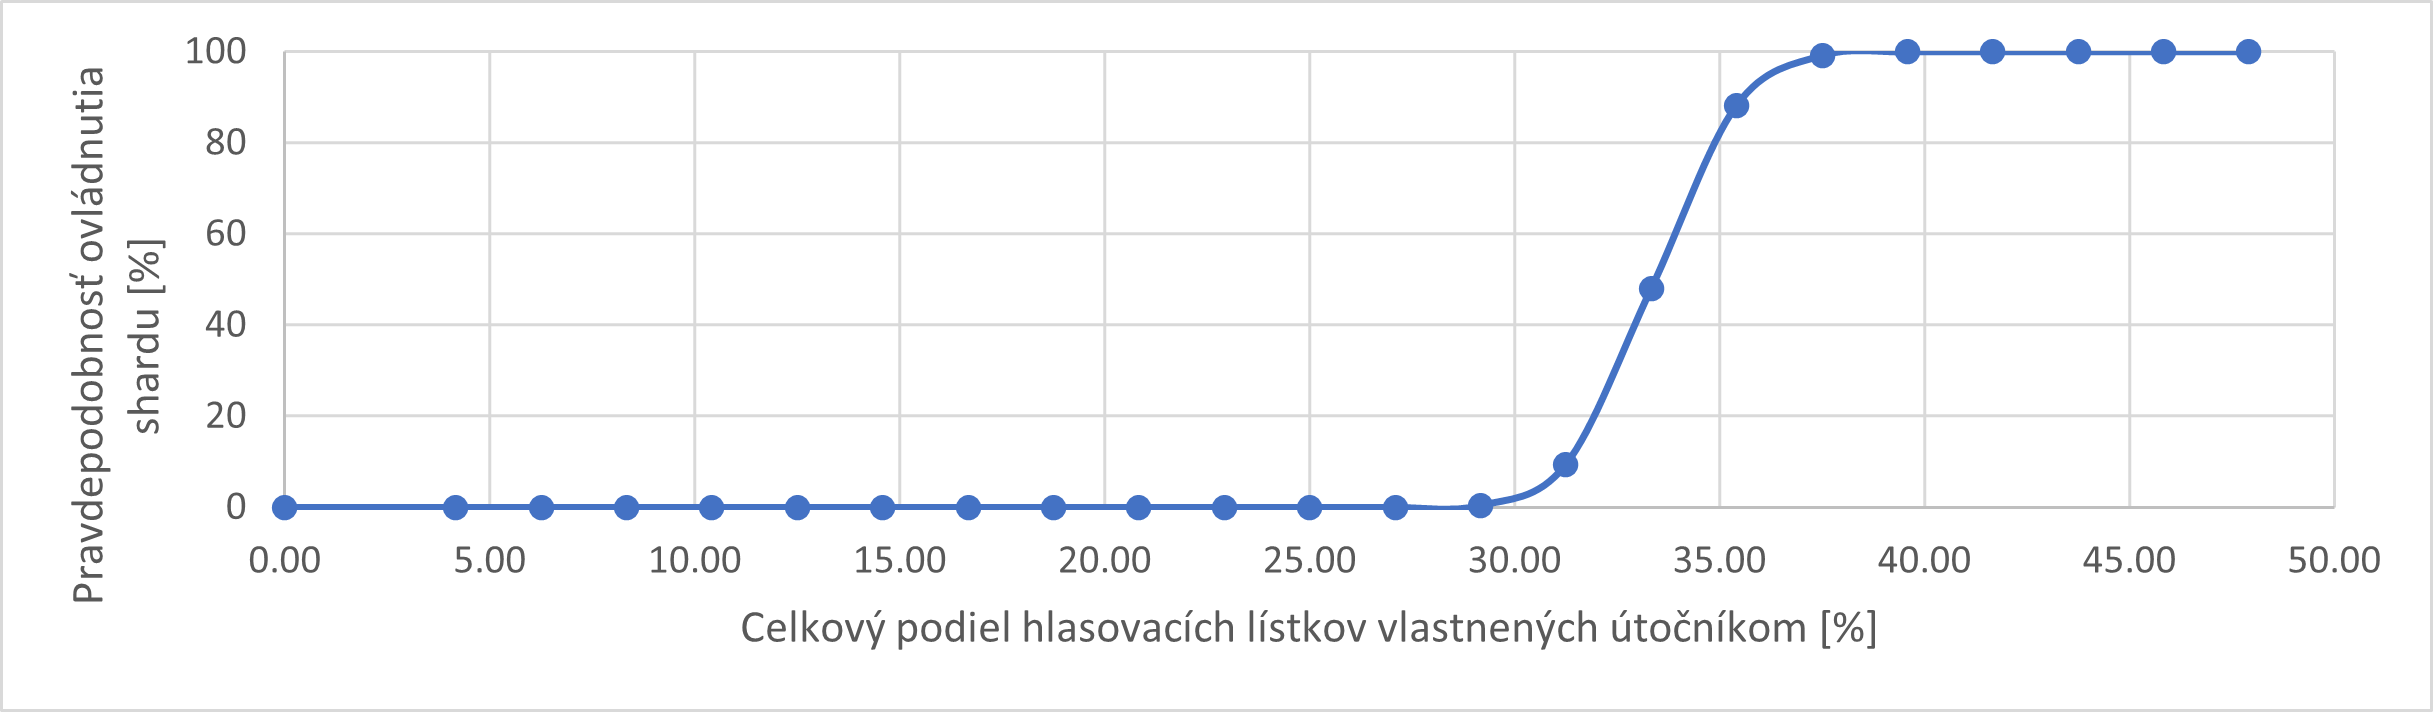
\includegraphics[width=\textwidth]{obrazky-figures/hypergeom-dist}
	\caption{Pravdepodobnosť ovládnutia jedného shardu útočníkom.}
	\label{img:hypergeom-dist}
\end{figure}

Obrázok~\ref{img:hypergeom-dist} ukazuje pravdepodobnosť ovládnutia jedného shardu v~závislosti na celkovom podiele hlasovacích lístkov vlastnených útočníkom. Tento výpočet je založený na už spomínanom hypergeometrickom rozdelení a parametroch BC Harmony~\cite{harmonyWp}. Môžeme vidieť, že útočník má zanedbateľnú pravdepodobnosť ovládnuť shard pokiaľ nevlastní približne $\frac{1}{3}$ z~celkového množstva hlasovacích lístkov. S~toho plynie, že shardingu v~tomto protokole neumožňuje útočníkovi využiť útok na podskupinu uzlov (viď sekcia~\ref{subsec:shard-attack}).

Harmony sharding používa algoritmus VDF na oneskorenie odhalenia náhodného čísla. %čím zabraňuje útoku na posledného objaviteľa (viď sekacia~\ref{subsec:lst-re-attack}).

\subsection{Komunikácie medzi shardami}
Autori deklarujú vysokú škálovateľnosť pomocou shardingu. Avšak samotné shardy sú všetky úzko závislé na beacon sharde z~dôvodu medzishardovej komunikácie. Každý nový blok v~ľubovoľnom sharde musí byť zaslaný do beacon shardu. Ten musí jeho hlavičku pomocou konsenzu uložiť do svôjho nového bloku a tento blok broadcastom poskytnúť všetkým ostatným shardom. Táto závislosť na beacon sharde môže potenciálne predstavovať výkonnostné úzke hrdlo. Aktuálne Harmony používa len 4 shardy a teda nie je overené ani jasné nakoľko bude tento protokol efektívny ak by pracoval s~desiatkami až stovkami shardov.

\subsection{Voľba vodcu FBFT}
Roľa vodcu v~protokole FBFT je dôležitá pretože, ak vodca nespolupracuje tak nie je možné vytvárať nové bloky. Voľba vodcu je skutočne náhodná a zároveň vodcom sa pravdepodobnejšie stávajú najväčší podielnici čo je z~pohľadu PoS bezpečné (viď útok~\ref{subsec:grinding-attack}). Avšak, vodca shardy sa nemení počas celej epochy (približne 18,2 hodiny) a všetci útočníci vedia, ktorý uzol je vodcom. S~tohoto hľadiska je možné počas celej epochy vykonávať DoS útok na vodcu, čím sa znemožní uzatvárať konsenzus (viď útok~\ref{subsec:leader-dos}). Samotný protokol Harmony tento útok nerieši a ochrana vodcu by preto musela byť vykonaná na sieťovej vrstve napríklad pomocou firewallu.

\chapter{Solana}\label{chap:solana}

Solana je BC technológia zameraná na vysokú priepustnosť transakcií. Klasická centralizovaná databáza dokáže mať priepustnosť až 710\,000 TPS na gigabitovej sieti s~priemernou veľkosťou transakcie 176\,B~\cite{solanaDoc}. Decentralizovaná databáza BC má dramaticky nižšiu priepustnosť. Tradičné PoW protokoly ako je Bitcoin (5~TPS) alebo Ethereum (15~TPS) dosahujú veľmi nízku priepustnosť%
\footnote{\url{https://academy.binance.com/en/glossary/transactions-per-second-tps}}.  V~kapitole~\ref{chap:harmony} bol popísaný PoS protokol Harmony, ktorý má už značne vyššiu priepustnosť (2\,000~TPS) dosiahnutú pomocou konceptu sharding. Autori Solana projektu deklarujú, že ich architektúra môže teoreticky dosiahnuť rovnakú priepustnosť ako centralizovaná sieť (710\,000~TPS) a to bez použitia konceptu sharding.

Solana poukazuje na to, že zníženie priepustnosti BC voči centralizovanej sieti je zapríčinené tým, že uzly v~sieti potrebujú synchronizovať čas a súčasne si navzájom nemôžu dôverovať. Solana projekt navrhol kryptografický algoritmus \textit{Proof-of-History} (viď sekcia~\ref{sec:solana-poh}) pomocou ktorého môže rýchlo a efektívne synchronizovať čas aj decentralizovaná sieť.

Solana konsenzus je založený na mechanizme PoS (sekcia~\ref{sec:solana-consens}) na ktorom funguje aj model motivácie tohoto protokolu (sekcia~\ref{sec:solana-motiv}). Sekcia~\ref{sec:solana-teor} na záver teoreticky zhodnocuje tento protokol z~hľadiska bezpečnosti a výkonnosti.

Ak nie je uvedené inak, všetky informácie v~tejto kapitole vychádzajú s~pôvodnej publikácie Solana~\cite{solanaWp} a oficiálnej dokumentácie tohoto projektu~\cite{solanaDoc}.

\section{Proof-of-History}\label{sec:solana-poh}

\textit{Proof-of-History} (ďalej len PoH) je kryptografický algoritmus, ktorý usporiada dátové záznamy v~čase tak ako vznikajú. Takýto algoritmus pomáha jednoznačne a nepopierateľne usporiadať transakcie a konsenzus hlasovania v~čase pre decentralizovanú sieť ako je BC. Dôkaz o~usporiadaní je založený na kryptografickej hash funkcii (pozri sekciu~\ref{subsec:hash}), ktorá spĺňa kritérium \textit{collision resistant}.

Obrázok~\ref{img:solana-poh} demonštruje princíp fungovania PoH. V~sieti vždy existuje jeden uzol, ktorý nazývame \textit{PoH generátor}. Ten neustále (najrýchlejšie ako dokáže) pridáva nové záznamy do hash pointer zoznamu (pozri sekciu~\ref{subsec:hash-pointer}). Pridávanie nových hashov do zoznamu je sekvenčné a podmienené existenciou predchádzajúceho hashu. Na samotné vytvorenie hashu sa používa algoritmus  VDF (\textit{Verifiable Delay Function~\cite{vdfBoneh}}). VDF garantuje, že vytvorenie nového hashu zaberie $k$ sekvenčných krokov pre nejaké $k$. Každý hash teda predstavuje časový bod a vzdialenosť dvoch hashov udáva časový interval.

Generátor je aktuálny vodca v~konsenzus protokole. Všetky transakcie a hlasy od rôznych klientov sú zasielané na generátor. Ten ich serializuje do PoH reťazca. Vždy keď generátor prijme dáta od klienta (transakciu alebo hlas) pridá ich do zoznamu. Ak práve nemá dáta tak generuje prázdny záznam. Na obrázku môžeme vidieť v~ktorých hashoch, alebo tiež časových momentoch, bola transakcia pridaná do reťazca.

Generátor priebežne rozosiela PoH sekvenciu do celej siete. Každý uzol potom môže jednoznačne určiť v~akom čase boli vygenerované transakcie a hlasy konsenzu. Synchronizácia v~BC Solana je založená na tomto koncepte.

Existuje teoretický útok pri ktorom útočník zmení poradie v~reťazci. Predpokladajme, že útočník pozná všetky transakcie a hlasy a má väčší výpočtový výkon než aktuálny generátor. Potom by dokázal vypočítať reťazec s~alternatívnym usporiadaním a publikovať ho skôr. Práve kvôli tomuto generátor reťazec vždy podpíše a až potom distribuuje (pozri sekciu~\ref{subsec:sign}).

\begin{figure}[bt]
	\centering
	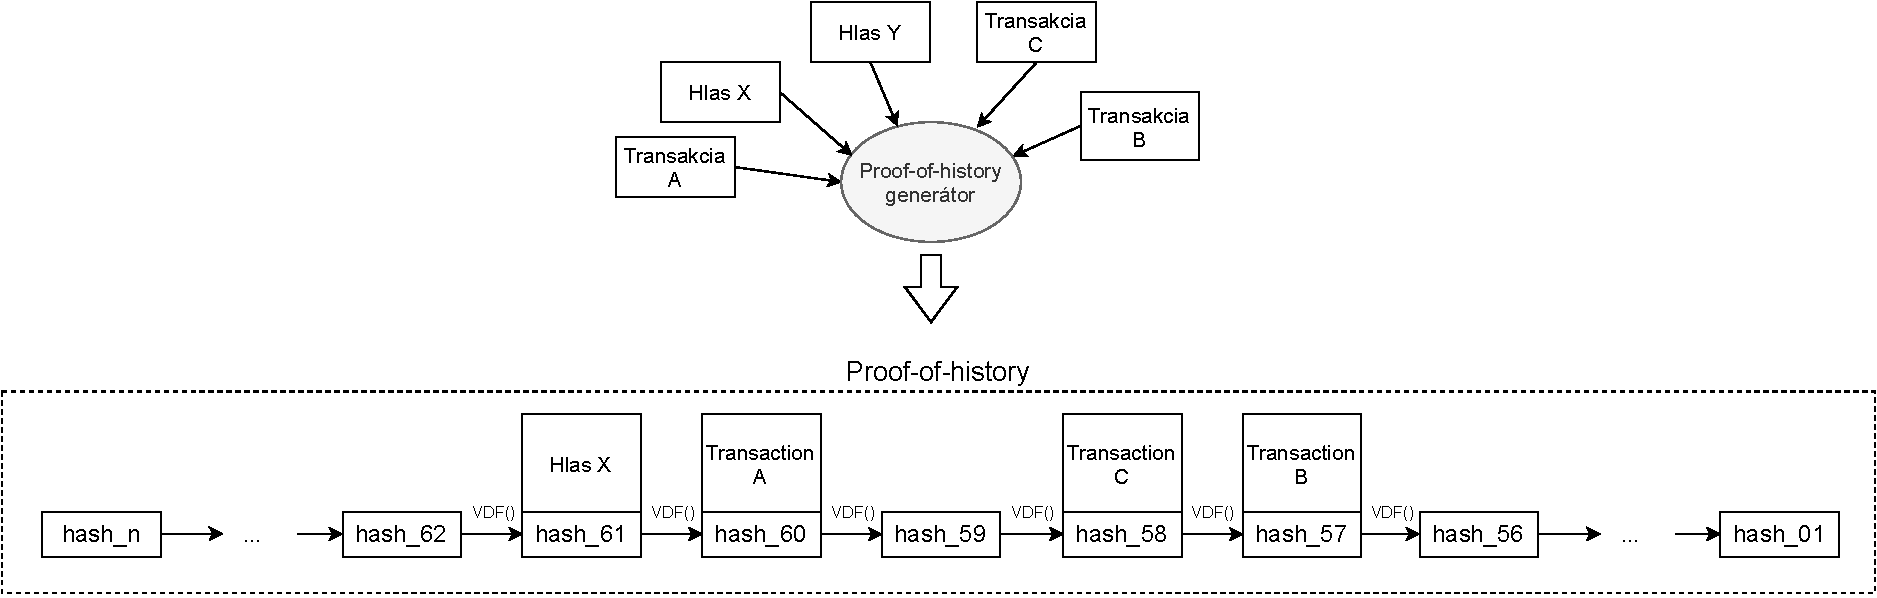
\includegraphics[width=\textwidth]{obrazky-figures/solana-poh-time}
	\caption{Reprezentácia času v~decentralizovanej sieti pomocou proof-of-history.}
	\label{img:solana-poh}
\end{figure}

\section{Konsenzus}\label{sec:solana-consens}

Solana navrhla konsenzus protokol, ktorý kombinuje Proof-of-History a Proof-of-Stake. Solana blockchain je tvorený PoH sekvenciou. Na uznesenie o~validnom stave PoH sekvencie sa používa konsenzus protokol, ktorý vychádza s~protokolu PBFT (pozri sekcii~\ref{subsec:pos-pbft}) a je popísaný v~sekcii~\ref{subsec:towerbft}. Do PoH reťazca pridáva nový blok vždy len aktuálny vodca, ktorý je určený rozvrhom vodcov (viď sekcia~\ref{subsec:pos-generator}). V~sekcii~\ref{subsec:solana-ldr-afk} je vysvetlený problém a riešenie výpadku PoH vodcu.

\subsection{Tower BFT}\label{subsec:towerbft}

Solana navrhla konsenzus protokol \textit{Tower BFT}, ktorý je založený na PBFT protokole:
\begin{enumerate}
	\item Klienti siete zasielajú transakcie na aktuálneho vodcu (PoH generátor).
	\item Vodca pridáva transakcie do PoH sekvencie a túto dátovú štruktúru distribuuje validátorom.
	\item Validátori overia transakcie v~PoH sekvencii a vykonajú ich v~stanovenom poradí. Takto získajú nový stav.
	\item V~špecifikovanom čase, po uplynutí určitého počtu PoH záznamov, pošlú validátori svoje hlasy vodcovi. Hlas je hash stavu validátora po vykonaní transakcií s~danej PoH sekvencie. Tento hash je navyše podpísaný privátnym kľúčom validátora. Takto validátor potvrdzuje, že súhlasí s~PoH sekvenciou ktorú podpísal. Ak zo sekveciou nesúhlasí, jednoducho svôj hlas nepošle.
	\item Vodca pridáva prijaté hlasy do PoH sekvencie.
	\item Validátori sledujú hlasy, ktoré sa následne vyskytujú v~PoH sekvencii. Každý validátor počíta hlasy a ak dosahujú $\frac{2}{3}$ celkového počtu validátorov, tak bol dosiahnutý konsenzus.
\end{enumerate}
Solana používa PoS a teda váha hlasu validátora je priamo úmerná jeho podielu. Pre konsenzus nie je nutné dosiahnuť $\frac{2}{3}$ celkového počtu hlasov validátorov, ale len toľko hlasov aby ich vlastníci vlastnili $\frac{2}{3}$ celkového podielu.

\subsection{Rozvrh vodcov Proof-of-History}\label{subsec:pos-generator}

Solana má obtiažnosť VDF nastavenú tak aby bolo možné vygenerovať PoH sekvenciu dlhú 160 hashov%
\footnote{\url{https://github.com/solana-labs/solana/blob/master/sdk/program/src/clock.rs}}. Jeden vygenerovaný hash nazývame \textit{tick}. Jeden vodca (PoH generátor) vygeneruje 64 tickov. Táto súvislá sekvencia sa nazýva slot. Jeden slot predstavuje približne 400 \,ms. Počas jedného slotu vygeneruje vodca jeden alebo žiaden blok. Nový vodca sa určí na základe už dopredu stanoveného rozvrhu. Rozvrh je stanovený na fixný počet slotov, ktorý voláme \textit{epocha}. Epocha trvá 420\,000 blokov čo sú približne 2 až 3 dni%
\footnote{Pozri poznámku 2}. Rozvrh na aktuálnu epochu sa vypočíta už v~predchádzajúcej. 

Samotný výpočet rozvrhu prebieha tak, že sa zoberú všetci vlastníci podielu, ktorý hlasovali v~posledných $n$ záznamoch PoH sekvencie, kde $n$ je konfigurovateľná konštanta. Pridelenie slotov je určené pseudo náhodným generátorom, ktorý je inicializovaný číslom aktuálneho slotu. Toto číslo je monotónne rastúci čítač v~čase. Algoritmus pseudo náhodne vyberie z~množiny možných kandidátov jedného vodcu pre každý slot nasledujúcej epochy pričom pravdepodobnosť voľby je priamo úmerná podielu daného validátora (PoS princíp). Voľbu PoH generátorov na celú epochu vykoná každý uzol lokálne. Tento algoritmus je deterministický a teda všetky uzly získajú rovnaký rozvrh.

\subsection{Nedostupnosť vodcu}\label{subsec:solana-ldr-afk}
Uzly v~Solana sieti tolerujú dočasnú stratu spojenia s~aktuálnym vodcom (PoH generátorom). Pri strate spojenia predpokladajú len prázdne záznamy, ktoré neobsahujú žiadne dáta. Takýto PoH reťazec si dokážu generovať aj sami, bez komunikácie zo sieťou, na základe posledného hashu minulého slotu.

Vetvenie v~Solana konsenze vzniká pri zmene vodcu. Nový vodca nemusel zachytiť hlasy uložené v~poslednom slote. Tento slot teda nahradí prázdnymi záznamami. Vetvenie slotu je teda binárne (vetva s~dátami a prázdna vetva). 

Každý validátor musí sledovať celý binárny strom možných vetiev a uchovávať si ich stav. Voľbu vetvy urobí validátor tak, že vodcovi v~danej vetve pošle svoj hlas čím vetvu potvrdí. Validátor potom nemôže hlasovať v~žiadnej inej vetve po dobu (pevný počet slotov) ktorá sa nazýva \textit{lockout}. Lockout perióda sa navyše zdvojnásobuje každým ďalším pridaným hlasom v~danej vetve až do maximálnej hodnoty (aktuálne je maximum 32 hlasov). Ak chce validátor hlasovať, za inú vetvu, musí počkať do konca periódy lockout. Následovne vykoná návrat späť (anglicky \textit{rollback}) do posledného spoločného stavu medzi starou a novou vetvou. Fungovanie a význam lockoutu a rollbacku je podrobnejšie popísaný v~sekcii~\ref{subsec:solana-branch}.

\section{Model motivácie}\label{sec:solana-motiv}

Hlasy v~konsenzus protokole sú zasielané v~podobe normálnych transakcií. Validátori teda musia za svoje hlasy v~konsenze platiť poplatky za transakcie. Všetky transakčné poplatky v~novom bloku sú rozdelené na dva fixne veľké diely $(\alpha ,\beta)$, ktoré sa môžu vývojom BC meniť a na počiatku sú nastavené na hodnotu $(\frac{1}{2},\frac{1}{2})$. Tvorca nového bloku (PoH generátor) získava za odmenu diel $\alpha$ a diel $\beta$ je zničený (anglicky \textit{burned}).

Validátori dostanú za validovanie globálneho stavu BC fixnú kompenzáciu. Táto odmena kompenzuje poskytnutie ich výpočtových zdrojov použitých na overovanie a hlasovanie. Kompenzácia je umelo vytvorená a spôsobuje infláciu hodnoty BC. Vyplácanie týchto odmien prebieha vždy za obdobie jednej epochy.

\subsection{Vetvenie}\label{subsec:solana-branch}
Hlasy v~každej vetve sa ukladajú do pomyselného zoznamu s~obmedzenou kapacitou na 32 položiek. Každý nový pridaný hlas do zoznamu zdvojnásobí lockout všetkých predošlých hlasov v~zozname. Keď zoznam dosiahne maximálnu kapacitu tak je najstarší hlas odstránený (FIFO) a majiteľ hlasu je odmenený.

Ešte pred tým ako je pridaný nový hlas do zoznamu tak je vykonaný \textit{rollback}. Rollback porovná časový slot pridania nového hlasu s~časovými slotmi v~ktorých končí lockout každého hlasu v~zozname. Ak niektorému hlasu skončil lockout v~slote, ktorý je skôr ako slot pridania nového hlasu tak je tento starší hlas odstránený zo zoznamu (LIFO).

S~toho vyplýva, že čím viac je vetva používaná, tím pravdepodobnejšie dosiahne ľubovoľný hlas koniec FIFO zoznamu a s~tým spojenú odmenu. Validátor ktorý chce maximalizovať svoje zisky je takýmto odmeňovaním motivovaný vybrať vetvu, ktorá je najpoužívanejšia a najstabilnejšia.

Validátor je potrestaný za súbežné hlasovanie v~rôznych vetvách. Ak hlasoval v~jednej vetve, tak je zaviazaný na hlasovanie len v~tejto vetve po dobu lockoutu. Ak validátor poruší lockout a bude mu to preukázané, budú mu odobrané jeho zdroje.

\section{Teoretická analýza}\label{sec:solana-teor}

Synchronizácia v~čase pomocou PoH umožňuje veľkú efektivitu a rýchlosť tohoto BC. Solana používa na uznesenie konsenzu obdobu PBFT protokolu, ktorú nazvala Tower BFT. PBFT má časovú zložitosť $O(n^2)$ pre $n$ uzlov, pretože broadcast vysiela vodca a následne aj validátori. Tower BFT má časovú zložitosť lineárnu pretože broadcast vysiela vždy len jediný uzol siete (PoH generátor). Avšak, Solana je závislá od vodcu pretože on jediný pridáva v~aktuálnom slote obsah do BC. Vodca sa každý slot mení, ale rozvrh vodcov je známy na viac ako dva dni dopredu. Útočník teda môže vykonať DoS útok na vodcu (viď útok~\ref{subsec:leader-dos}).

Útočník nemôže ovplyvniť voľbu vodcu v~svoj prospech inak ako vložením väčšieho množstva zdrojov pretože inicializačný vektor pre pseudo náhodnú voľbu je preňho neovplyvniteľný (viď sekcia~\ref{subsec:pos-generator}).

Potenciálnou nevýhodou tohoto BC je aj fakt, že každý validátor musí byť neustále dostupný.

\chapter{Ouroboros}\label{chap:ouroboros}

Ouroboros je PoS protokol, ktorý je používaný v~kryptomene Cardano. Autori Cardano deklarujú%
\footnote{\url{https://www.youtube.com/watch?v=Ja9D0kpksxw}}, že všetky technológie, protokoly a algoritmy použité v~ich BC sú vyberané koncepciou recenzného hodnotenia. Inak povedané, Cardano používa technológie, ktoré boli vedecky prezentované a kladne prijaté komunitou okolo technológie BC. V~zmysle tohoto konceptu bol ako PoS protokol zvolený práve Ouroboros. Tento projekt má za cieľ formálne dokázať bezpečnosť ich konsenzus protokolu. V~tejto kapitole je vysvetlený princíp fungovania protokolu Ouroboros na základe oficiálnej publikácie tohoto projektu~\cite{ouroborosWp}.

\section{Konsenzus}
Ouroboros konsenzus je uznesený ak sa viac ako 50\,\% (majorita vlastníkov podielu) zhodne na stave BC.

\subsection{Synchronizácia v~čase}
Protokol Ouroboros pracuje s~časom v~dvoch jednotkách. Najmenšia časová jednotka je \textit{slot}. Za jeden slot je vytvorený maximálne jeden blok (čas potrebný na komunikáciu v~decentralizovanej peer-to-peer sieti). Slot je najmenšia časová jednotka na synchronizáciu uzlov v~sieti. 

Druhou (väčšou) časovou jednotkou je \textit{epocha}, ktorú tvorí pevný počet slotov $R$. Pre Cardano%
\footnote{\url{https://developers.cardano.org/docs/stake-pool-course/introduction-to-cardano/}} je $R$ rovné 432\,000 slotom (približne päť dní).

\subsection{Protokol}\label{subsec:ouroboros-protocol}
Pre každý slot je určený vodca podľa dopredu známeho rozvrhu. Proces určenia rozvrhu vodcov je popísaný v~sekcii~\ref{sec:ouroboros-slot-leader}. Vodca môže ako jediný vytvoriť blok v~danom slote. 
Blok obsahuje sekvenčné číslo slotu a je podpísaný privátnym kľúčom jeho tvorcu. Overenie validnosti bloku prebieha na základe čísla slotu zapísaného v~hlavičke tohoto bloku. Každý validátor sa pozrie do rozvrhu a určí kto má byť vodca pre daný slot. Následne overí, že blok je podpísaný práve týmto vodcom.

Každý uživateľ vykonáva nasledujúce činnosti:
\begin{itemize}
	\item Zber validných transakcií zo siete.
	\item Zber všetkých BC, ktoré sú distribuované sieťou a kontrola ich validity (sekvencia blokov má len rastúce sekvenčné čísla slotov, transakcie sú validné, blok je vytvorený správnym vodcom). Každý udržiava najdlhší validný BC (rovnaký princíp ako Bitcoin).
	\item Ak je uživateľ aktuálny vodca, tak vytvorí nový blok z~transakcií ktoré získal. Blok pridá na koniec BC a distribuuje ho. Je dôležité podotknúť, že vodca nemusí vždy publikovať nový blok a teda slot môže byť "prázdny". Avšak jeden slot môže publikovať maximálne jeden blok.
\end{itemize}

\subsection{Schéma delegovania}\label{subsec:ourobors-delegation}
Ouroboros protokol vyžaduje aby bol vlastník podielu neustále online, ak sa chce podieľať na tvorbe nových blokov. Táto požiadavka je príliš nepraktická a nerealistická. Preto Ouroboros poskytuje schému delegovania práva na generovanie blokov. Ak je vlastník zvolený za vodcu slotu, môže tento post delegovať inému užívateľovi (delegátovi). Tento užívateľ teda vytvorí nový blok namiesto skutočného vodcu slotu. Avšak, vlastník podielu deleguje len svoje právo na tvorbu bloku. Delegát nemá možnosť manipulovať zo zdrojmi, ktoré nie sú jeho. Koncept delegovania umožňuje zoskupovať podielnikov do väčších celkov (anglicky \textit{stake pools}). 

Delegovanie je zabezpečené pomocou kryptografického konceptu \textit{Proxy Signatures}~\cite{proxySig}. Skutočný vodca slotu si vytvorí kľúč na delegovanie digitálneho podpisu (anglicky \textit{proxy signing key}), ktorým delegát podpíše vytvorený blok. Proxy kľúč kryptograficky zabezpečuje, že ktokoľvek môže overiť nasledujúce jeho vlastnosti:
\begin{itemize}
	\item Verifikácia: Identita tvorcu proxy kľúča a identita delegáta, ktorému bol vystavený.
	\item Prevencia pred zneužitím: Tento kľúč je časovo limitovaný pretože jeho tvorca definuje presný slot v~ktorom platnosť kľúča expiruje. 
\end{itemize}

\section{Vodca slotu}\label{sec:ouroboros-slot-leader}

Rozvrh vodcov pre jednotlivé sloty sa vytvára na obdobie jednej epochy a je známy už na jej začiatku. Každý užívateľ si môže vypočítať vodcov ($U_1, U_2,  ..., U_R$) pre jednotlivé sloty ($1, 2, ..., R$) v~aktuálnej epoche pomocou funkcie $L(stake, rnd)$, kde:
\begin{itemize}
	\item $stake$: Rozdelenie podielu (anglicky \textit{stake distribution}) v~predchádzajúcej epoche. Rozdelenie podielu sa vezme z~$k$-tého slotu v~predchádzajúcej epoche, kde $k$ je parametricky nastaviteľná konštanta.
	\item $rnd$: Dostatočne dlhý a skutočne náhodný reťazec $rnd \in \{0,1\}^*$ vytvorený pomocou distribuovanej generácie náhodnosti v~minulej epoche. Aby bol reťazec považovaný za skutočne náhodný, musí byť produktom kryptograficky bezpečného výpočtu všetkých zainteresovaných strán. Ouroboros používa pre tento účel kombináciu algoritmov \textit{Coin Tossing} (viď~\ref{subsec:ouroboros-coin-tossing}) a PVSS (viď~\ref{subsec:ouroboros-pvss}).
\end{itemize}
Funkcia $L$ z~náhodného reťazca $rnd$ pomocou deterministického algoritmu určí rozvrh pričom pravdepodobnosť zvolenia za vodcu je priamo úmerná podielu daného užívateľa. Pri voľbe vodcu sa teda uplatní PoS princíp (napríklad, ak v~predchádzajúcej epoche vlastní užívateľ 2\,\% podielu tak má v~aktuálnej epoche práve 2\,\% šancu stať sa vodcom slotu).

\subsection{Coin Tossing protokol}\label{subsec:ouroboros-coin-tossing}

\textit{Coin Tossing}~\cite{coinFlipBlum} protokol umožňuje dvom stranám (uvažujme Alicu a Boba) vytvoriť rovnomerne náhodný reťazec. Protokol funguje nasledovne:
\begin{enumerate}
	\item Alica vygeneruje náhodný reťazec $u_1 \in \{0,1\}^*$ a navzorkuje z~neho náhodnosť $r$. Následne pošle Bobovi dôkaz $Commit(r,u_1)$ tejto hodnoty, ktorý ju však neodhaľuje.
	\item Bob vygeneruje svoj náhodný reťazec $u_2 \in \{0,1\}^*$ a pošle ho Alici. 
	\item Alica odhalí $u_1$ zaslaním kryptografického dôkazu $Open(r,u_1)$. Bob si môže overiť, že $Open(r,u_1)$ odpovedá $Commit(r,u_1)$ a teda Alica určite nepozmenila pôvodné $u_1$.
	\item Obe strany vypočítajú výstupnú náhodnosť $u = u_1 \oplus u_2$.
\end{enumerate}

Ouroboros používa pre vytvorenie náhodného reťazca rozšírenie protokolu \textit{Coin Tossing}, ktoré uvažuje viac ako dve strany a to pomocou algoritmu PVSS (viď sekcia~\ref{subsec:ouroboros-pvss}).

\subsection{PVSS}\label{subsec:ouroboros-pvss}

PVSS (\textit{Publicly Verifiable Secret Sharing})~\cite{pvssFeldman} je kryptografická schéma, ktorá umožňuje rozdeliť tajomstvo $\sigma$ na $n$ dielov. Pôvodné $\sigma$ je možné zrekonštruovať pokiaľ je poškodených maximálne $t$ dielov (nedostupných alebo úmyselne pozmenených útočníkom), kde $t$ je nastaviteľný parameter. Schéma definuje nasledujúce dve funkcie:
\begin{itemize}
	\item $Deal(n, t, \sigma) = (\sigma_1, \sigma_2, ..., \sigma_n)$, kde vstupy $n$, $t$ a $\sigma$ sú počet dielov na vygenerovanie, maximálny počet poškodených dielov a vstupné tajomstvo. Výstupom funkcie sú diely tajomstva.
	\item $Rec(\sigma_1, \sigma_2, ..., \sigma_n) = \sigma$, kde vstupom sú diely vytvorené funkciou \textit{Deal} a výstupom je rekonštrukcia pôvodného tajomstva $\sigma$ ak platí, že maximálne $t$ vstupných dielov je poškodených.
\end{itemize}

\subsection{Protokol pre generovanie distribuovanej náhodnosti}\label{subsec:ouroboros-rnd}
 
Nech dĺžka epochy $e_j$ je $R=10k$ slotov a vodcovia slotov $1,2,...,R$ sú $U_1, U_2, ..., U_R$ (vodcovia nemusia byť nutne rôzny). Potom protokol pre distribuované generovanie náhodnosti pre epochu $e_{j+1}$ je definovaný následovne:
\begin{enumerate}
	\item Fáza záväzku: Ide o~prvých $4k$ slotov. Každý vlastník podielu $U_i$, pre $1 \leq i \leq R$, vygeneruje náhodný reťazec $u_i$ a navzorkuje z~neho náhodnosť~$r_i$. Následne rozdelí tajomstvo $u_i$ na diely $\sigma_1, \sigma_2, ..., \sigma_R$ pomocou $Deal(R,R/2,u_i)$. Každé $\sigma_j$, pre $1 \leq j \leq R$, zašifruje verejným kľúčom užívateľa $U_j$. Vlastník podielu $U_i$ uloží do BC zašifrované diely tajomstva a zároveň kryptografický dôkaz $Commit(r_i, u_i)$. Všimnime si, že $t$ vo funkcii $Deal$ je nastavené na $R/2$. To znamená, že na rekonštrukciu tajomstva je potrebná majorita vlastníkov podielu.
	\item Fáza odhalenia: Po uplynutí $4k$ slotov, každý účastník odstráni posledných $k$ slotov a vo zvyšku identifikuje držiteľov podielu. Ak majorita držiteľov podielu publikovala $Commit$, tak začína fáza odhalenia. V~opačnom prípade protokol zastaví. Následne každý vlastník podielu $U_i$, pre $1 < i \leq R$, odhalí tajomstvo $u_i$ tým, že vloží do BC $Open(r_i, u_i)$.
	\item Fáza obnovy: Po uplynutí $8k$ slotov, každý účastník odstráni posledných $k$ slotov a vo zvyšku identifikuje všetkých držiteľov podielu, ktorý odhalili ich tajomstvo $u_i$ (overenie $Commit(r_i, u_i)$ voči $Open(r_i, u_i)$). Ak nejaký nepoctivý účastník $U_x$ nezverejnil $Open$ k~svojmu $Commit$, tak všetci poctivý účastníci zverejnia  $\sigma_1, \sigma_2, ..., \sigma_n$, ktoré patria k~tajomstvu $u_x$. Ak bude poctivých účastníkov viac ako $t$ (majorita), tak bude možné použiť $Rec(\sigma_1, \sigma_2, ..., \sigma_n)$ na rekonštrukciu tajomstva $u_x$.
	\item Nová epocha: Každé tajomstvo $u_i$, pre $1 \leq i \leq R$, je teraz už verejne známe. Výsledná náhodnosť pre epochu $e_{j+1}$ vypočíta každý účastník ako $u_1 \oplus u_2 \oplus ... \oplus u_R$.
\end{enumerate}


\section{Model motivácie}

Ouroboros motivuje účastníkov protokolu chovať sa poctivo pomocou modelu odmeňovania. Transakcie zahrnuté do blokov obsahujú poplatky (anglicky \textit{transaction fee}), ktoré tvorcovia transakcií musia zaplatiť podielnikom. Samotné odmeny sa počítajú a vyplácajú za obdobie jednej epochy.

Celkový fond odmien $T_{all}$ pre epochu $e_j$ je daný rovnicou~\ref{eq:ouroboros-reward-pool}, kde R je počet slotov v~epoche a $T_i$ sú všetky poplatky za transakcie v~slote $i$. Ak sa ľubovoľná transakcia vyskytne vo viacerých blokoch, tak je poplatok uvažovaný len pri jej prvom výskyte.
\begin{equation}\label{eq:ouroboros-reward-pool}
	T_{all} = \sum_{i=1}^{R}\sum_{k \in T_i}t_k
\end{equation}

V~epoche $e_j$ uvažujme vodcov $U_1, U_2, ..., U_R$ pre sloty $1, 2, ..., R$ a všetkých podielnikov označme ako množinu $\mathbf{P}$. Potom $i$-tý podielnik $p_i \in \mathbf{P}$ dostane za epochu $e_j$ odmenu $\alpha_i$ určenú rovnicou~\ref{eq_ouroboros-reward}.
\begin{equation}\label{eq_ouroboros-reward}
	\alpha_i = \frac{|\{ k\,|\,p_i = U_k \}|}{R}T_{all}
\end{equation}

Odmena podielnika teda nevychádza z~transakcií, ktoré sú pridané do BC v~jeho vodcovských slotoch, ale je vždy priamo úmerná jeho podielu. Tento model motivácie teda odmeňuje podielnikov nie za vytváranie blokov, ale za samotné vlastníctvo podielu.

\section{Teoretická analýza}

Ouroboros používa pravidlo najdlhšieho reťazca (anglicky \textit{longest chain rule}) na voľbu správneho reťazca v~prípade vetvenia. Útočník nemôže efektívne vytvoriť dostatočne dlhý alternatívny reťazec pretože jednotlivé bloky musia byť podpísané správnym vodcom daného slotu. Útočník by teda potreboval privátne kľúče všetkých vodcov slotov od bodu v~ktorom by chcel vytvoriť vetvenie.

Voľba vodcu slotu je skutočne náhodná. Voľbu vodcu nie je možné ovplyvniť inak ako investovaním väčšieho množstva zdrojov do BC (viď sekcia~\ref{subsec:ouroboros-rnd}). Tento princíp je z~hľadiska PoS správny.

Útok zdvojenia výdavkov nie je možné uskutočniť (dôkaz viď~\cite{ouroborosWp}, kapitola~5, teorém~5.5).

\chapter{Teoretické porovnanie protokolov}\label{chap:protocol-comparison}

Teoretická analýza protokolov Harmony (kapitola~\ref{chap:harmony}), Solana (kapitola~\ref{chap:solana}) a Ouroboros (kapitola~\ref{chap:ouroboros}) je zhrnutá v~tabuľke~\ref{img:protocol-comparison}. Tabuľka porovnáva tieto tri protokoly z~hľadiska shardingu, synchronizácie v~čase, tvorby nového bloku, modelu motivácie, vetvenia a odolnosti voči rôznym útokom.

Môžeme vidieť, že len protokol Harmony používa škálovatelnosť pomocou shardingu. Pre ovládnutie jedinej shardy útočník potrebuje viac ako $\frac{1}{3}$ celkového podielu.

Na synchronizáciu v~čase používajú všetky tri protokoly koncept epochy a slotu. Z~tohoto hľadiska je možné poukázať na vysokú rýchlosť Solana protokolu, ktorý dokáže za približne pol hodiny vygenerovať 420\,000 blokov. Protokol Harmony aktuálne generuje za rovnaký čas len približne 900 blokov a Ouroboros približne 1\,800 blokov.

Pre vytvorenie nového bloku potrebujú všetky tri protokoly určiť uzol, ktorý blok vytvorí (tzv. vodcu). Túto dôležitú roľu prideľujú všetky protokoly náhodnou voľbou. Harmony a Ouroboros používajú algoritmus na vytvorenie distribuovanej náhodnosti a teda zabraňujú útočníkom ovplyvňovať výsledok volieb. Solana používa pseudonáhodný generátor, ktorý je inicializovaný číslom aktuálneho slotu (neovplyvniteľná monotónne rastúca hodnota). Pravdepodobnosť zvolenia za vodcu je vždy priamo úmerná podielu (princíp PoS). Ouroboros používa pravidlo \textit{longest chain rule} na určenie správneho reťazca. Uznesenie konsenzu má teda konštantnú časovú zložitosť vzhľadom k~počtu uzlov siete. Harmony a Solana používajú hlasovacie protokoly na uznesenie konsenzu pre novo publikovaný blok. Časová zložitosť hlasovania je potom lineárna vzhľadom k~počtu uzlov.

Solana umožňuje potenciálne binárne vetvenie pre každý nový blok. Každý validátor si musí udržiavať všetky možné vetvy čo kladie nemalé nároky na zdroje validátorov. Avšak, Solana zamedzuje podielnikom hlasovať v~rôznych vetvách súčasne pod trestom straty všetkých zdrojov.

Z~hľadiska potenciálnych útokov sa zdajú Harmony a Solana náchylné k~útoku na vodcu. V~oboch prípadoch je na celú epochu dopredu známe kto je vodcom. Útočník potom môže vykonať DoS útok na vodcu bez ktorého protokol nepublikuje žiadny nový obsah do BC. V~prípade Harmony je dokonca rovnaký vodca po dobu 18 hodín.

Na celkové ovládnutie Harmony alebo Solana BC je potrebné vlastniť viac ako $\frac{2}{3}$ podielu (na prekazenie konsenzu postačuje viac ako $\frac{1}{3}$). Ouroboros požaduje na ovládnutie konsenzu majoritu podielu (viac ako $\frac{1}{2}$).

\begin{figure}[H]
	\centering
	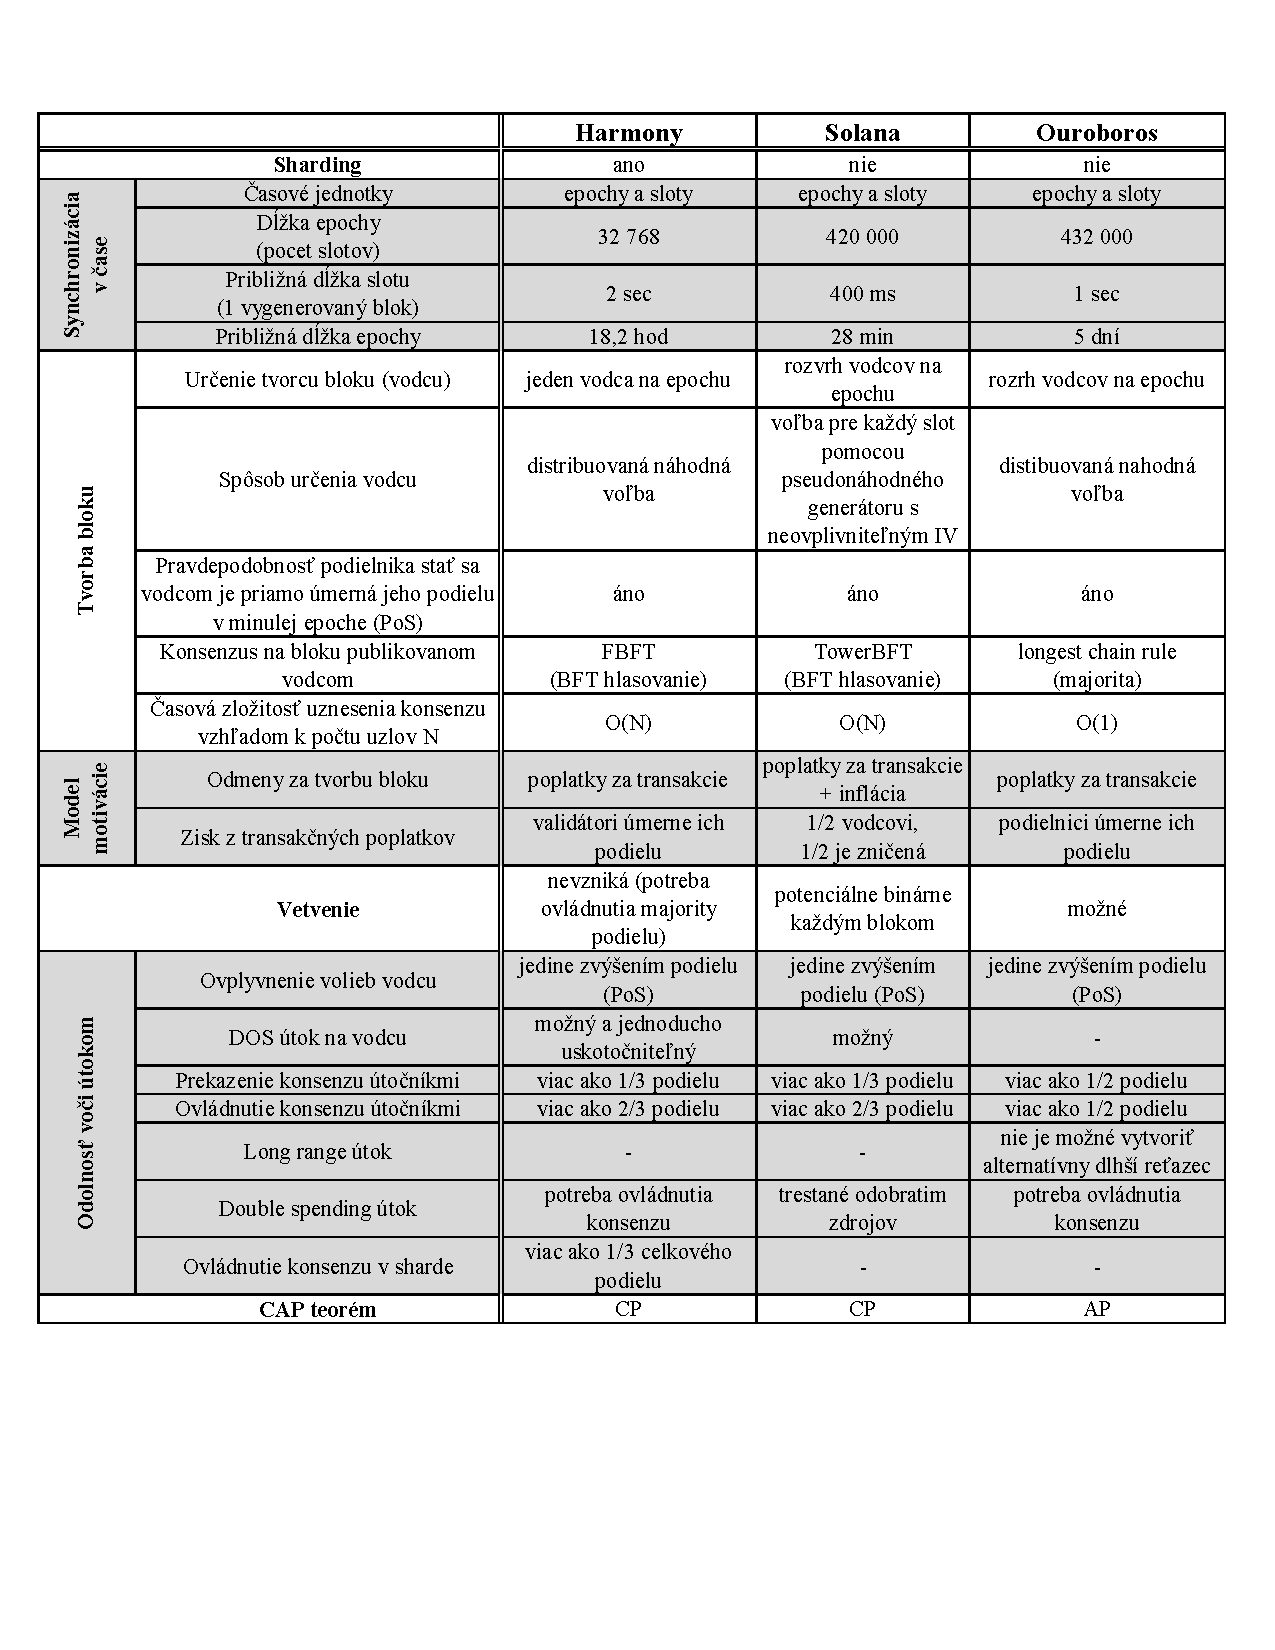
\includegraphics[width=\textwidth]{obrazky-figures/protocol-comparison}
	\caption{Porovnanie vlastností zvolených troch Proof-of-Stake protokolov.}
	\label{img:protocol-comparison}
\end{figure}


\chapter{Prehľad existujúcich simulátorov}\label{chap:simulators-overview}

Pre simuláciu zvolených PoS protokolov nebude vytvorený úplne nový simulátor. Simulácia celej technológie BC s~dostatočne presným model je rozsiahla úloha nad rámec tejto práce. Navyše už boli vytvorené simulačné nástroje, ktoré simulujú rôzne BC protokoly. K~týmto simulátorom existujú práce ktoré experimentálne vyhodnotili ich presnosť (viď\cite{simulatorCompar, fanPerfEval}). Preto bude použitý jeden s~týchto nástrojov. Zvolený nástroj bude následne upravený a rozšírený tak aby bolo možné simulovať zvolené PoS protokoly. 

Táto kapitola analyzuje niekoľko aktuálne dostupných simulátorov BC. V~závere kapitoly je vykonané porovnanie najvhodnejších nástrojov a je zvolený jeden pre ďalšiu prácu.

%Použiť túto prácu na porovannie~\cite{simulatorCompar}

%Caw, keď sa mrkneš na porovnanie simulátorov ktoré mám v práci, tak si môžeš všimnúť, že niektoré z iných simulátorov sú tvorené iba pre PoW ale taktiež u väčšiny nemáš dostupný zdroják alebo je o nich dokonca len napísaná práca a ani si ich nevieš vyskúšať. Bitcoin Simulator mal už naimplementovaný prenos správ a taktiež ukladanie blokov do ledgeru, čo mi celkom vyhovovalo a len som to rozšíril o tie protokoly, no napr. chalan predo mnou sa to snažil v NS3 urobiť komplet celé aj s výmenou transakcií, ktorá v mojom simulátore chýba a simulujem tam len časovým oneskorením pri dobe prenosu veľkosť jednotlivých blokov. Dávaj bacha ale akým spôsobom robíš niektoré operácie, lebo môj simulátor bol v konečnom dôsledku dosť pomalý a na simulácie som používal 64 CPU a 150GB RAM v metacentre, kde sa mi tesne pred odovzdaním podarilo ale vyčerpať fairshare skore, čiže na doknčenie práce som musel ešte použiť kamarátov účet  NS3 je ale podľa mňa celkom dosť vhodný spôsob nakoľko ti umožňuje simulovať rozsiahle siete a rôzne správanie v nich.. taktiež ak by sa ti podarilo spraviť dobrý simulátor, tak by bolo fajn ho hodiť ako public tool v NS3, čo určite ocení oponent ale aj komisia. Inak je to celkom jednoduchá téma a len to znie zložito, no určite na ňu nekašli lebo kódiť to len v posledných mesiacoch neni dobrý nápad  Btw, výhoda tej témy je to, že ak máš dobre vybraté protokoly, tak niektorí profáci nevedia ako majú správne fungovať a chalan predomnou dostal A za simulátor, čo nerobil ani zďaleka to čo mal.. z 3 protokolov mal naimplementované 2 a aj tie úplne mimo (pri Algorande mu chýbalo VRF a podobne), testy  bezpečnosti ani neskúsil a testy výkonu boli len také na pár riadkov, čiže reálne nesplnené zadanie ale tým, že tomu oponent nerozumel, tak si myslel, že je to spravené perfektne


\section{SimBlock}

SimBlock je simulátor založený na diskrétnej simulácii. Je implementovaný v~programovacom jazyku Java a jeho zdrojový kód je voľne dostupný (anglicky \textit{open source})~\footnote{Apache License, Version 2.0}. Simulátor podporuje PoW protokoly Bitcoin, Litecoin, a Dogecoin. Avšak umožňuje aj modulárne zmeniť konsenzus protokol. Posledná stabilná verzia pridala jednoduchú implementáciu PoS konsenzu~\footnote{\url{https://github.com/dsg-titech/simblock/releases/tag/v0.8.0}}.

Autori tohoto projektu v~rámci vyhodnocovania presnosti simulátora vykonali experiment ktorý porovnal ich prácu s~podobným už existujúcim simulátorom. Obe simulácie spustili s~rovnakými parametrami a to pre protokoly Bitcoin, Litecoin, a Dogecoin. Výsledky oboch simulátorov boli veľmi podobné. Na základe tohoto experimentu autori zhodnotili, že ich simulátor napodobuje reálne BC systémy s~porovnateľnou presnosťou ako podobné simulátory.

Autori ďalej navrhli úpravu algoritmu na voľbu susedných uzlov (anglicky \textit{neighbor node selection algorithm}) v~protokole Bitcoin. Navrhnutú úpravu odsimulovali a vyhodnotili, že ich vylepšenie algoritmu zvyšuje priepustnosť transakcií. Touto simuláciou bol demonštrovaný význam tohoto simulačného nástroja a to je zlepšovanie BC protokolov z~hľadiska výkonnosti a bezpečnosti pomocou simulácie.~\cite{simblockWp}

Výhodou tohoto simulačného nástroj je schopnosť simulovať aj rozsiahle siete s~viac ako 10\,000 uzlami. Ďalšou výhodou je, že simulácia ustanovuje medzi uzlami priame spojenie (anglicky \textit{point-to-point}) uvažujúce geografickú lokalitu jednotlivých uzlov. Simulácia teda umožnuje zohľadňovať sieťové oneskorenie (anglicky \textit{latency}) a šírku pásma (anglicky \textit{bandwidth}). 

Na druhú stranu, simulátor predpokladá, že všetky uzly sú poctivé. V~aktuálnej implementácii teda neumožňuje experimentovanie so zlomyseľným správaním niektorých uzlov. Pre analýzu útokov ako je double-spending alebo selfish-mining by bolo potrebné tento simulačný nástroj rozšíriť. Ďalšou možnou nevýhodou je, že simulácia prebieha na úrovni blokov a propagácia transakcií zatiaľ nie je uvažovaná.~\cite{fanPerfEval}

\section{Bitcoin Simulator}

Bitcoin Simulator je open source~\footnote{\url{https://arthurgervais.github.io/Bitcoin-Simulator/index.html}} simulačný nástroj implementovaný v~programovacom jazyku C++. Simulátor je postavený nad platformou NS-3~\footnote{\url{https://www.nsnam.org/}}, ktorá slúži na diskrétnu simuláciu Internetových systémov. Na tejto platforme je teda postavená simulácia peer-to-peer siete BC. Tento simulátor je určený a bol vyvinutý na experimentovanie s~PoW protokolmi. Aktuálne podporuje protokoly Bitcoin, Litecoin, a Dogecoin. Simulátor teda nepodporuje PoS konsenzus. Avšak v~minulosti už bol tento nástroj použitý treťou stranou, ktorá rozšírila implementáciu o~PoS protokoly Algorand, Casper FFG a Gasper (viď~\cite{borcikDp}). 

Autori simulátoru vykonali experiment na vyhodnotenie presnosti ich nástroja. Tri vyššie spomenuté protokoly boli simulované na rozsiahlej sieti a boli namerané mediány propagačného času bloku. Mediány získané zo simulácie boli relatívne podobné mediánom skutočných sietí postavených na týchto troch protokoloch. S~tohoto hľadiska bol simulátor vyhodnotený ako pomerne presný.~\cite{btcSimulatorWp}

Medzi výhody tohoto simulačného nástroja patrí jeho rozsiahlosť, ktorá poskytuje veľkú škálu vstupných parametrov a taktiež veľké množstvo nameraných výstupných metrík. Z~hľadiska simulácie PoW protokolov umožňuje simulátor rozlišovať rôzne typy uzlov (bežný uzol a miner uzol). Rozlišovanie rôznych uzlov umožňuje tomuto nástroju simulovať aj zlomyseľné chovanie niektorých uzlov. Tento simulátor teda umožňuje analyzovať aj bezpečnosť PoW konsenzu z~hľadiska ťažby blokov (útoky selfish-mining a double-spending).~\cite{fanPerfEval}

\section{BlockSim}\label{sec:blocksim}

BlockSim je open source~\footnote{\url{https://github.com/maher243/BlockSim}} simulátor vytvorený v~programovacom jazyku Python3 určený na diskrétnu simuláciu BC. Autori definujú tri základné ciele tohoto simulátora: všeobecnosť, rozširovateľnosť a jednoduchosť. Všeobecnosť architektúry simulátora umožňuje simuláciu veľkého množstva BC systémov. Simulátor by malo byť možné jednoducho rozšíriť o~ďalšie protokoly. Oba predošlé ciele majú viesť k~tomu aby bol tento nástroj jednoduchý na použitie. 

Simulátor poskytuje všeobecnú abstrakciu BC, ktorú autori nazvali \textit{base model}. Base model je zdieľaná vrstva pre všetky konkrétne protokoly pretože pokrýva všetky základné prvky BC (uzly, transakcie, bloky, reťazec blokov, fork reťazca). Nad touto vrstvou je potom možné vytvoriť implementáciu konkrétnych protokolov. Autori demonštrovali túto flexibilnú architektúru tak, že vytvorili nad base modelom simuláciu dvoch PoW protokolov (Bitcoin a Ethereum). Simulátor by teda mal byť priamočiaro rozšíriteľný aj o~simuláciu PoS protokolov. Avšak takáto simulácia by neumožnila analýzu špecifickej sekvencie správ PoS konsenzu.~\cite{blocksimWp}	

Najväčšou výhodou tohoto simulátoru je jeho jednoduchá architektúra, ktorá umožňuje rozšíriteľnosť o~ďalšie BC protokoly. Simulátor pokrýva sieťovú, dátovú a konsenzus vrstvu. Z~hľadiska sieťovej vrstvy je možné simulovať oneskorenie a šírku pásma pomocou geografickej distribúcie uzlov siete. Ďalšou výhodou je pomerne veľké množstvo konfigurovateľných vstupných parametrov simulácie. 

Naopak nevýhodu simulátoru je, že nedokáže efektívne simulovať rozsiahle siete. Tento simulátor sice podporuje simulácie transakcií avšak tento proces je limitovaný, keďže implementácia neobsahuje žiaden model účtov (napríklad UTXO~\footnote{\url{https://river.com/learn/terms/u/unspent-transaction-output-utxo/}} pre Bitcoin).~\cite{fanPerfEval}

\section{VIBES}

VIBES je open source~\footnote{\url{https://github.com/i13-msrg/vibes}} nástroj pre simuláciu BC technológie. Simulátor implementuje výhradne PoW konsenzus. Podľa autora je možná implementáciu rozšíriť o~PS konsenzus. Tento simulátor je zameraný na všeobecnejšiu simuláciu BC v~peer-to-peer sieti a neobsahuje implementáciu žiadneho konkrétneho protokolu.~\cite{vibesWp}

Výhodu tohoto nástroja je možnosť simulácie škodlivých uzlov. Simulátor je teda možné použiť na bezpečnostnú analýzu konsenzus protokolov. Ďalej, je podporovaná simulácia na úrovni dát (transakcie). Avšak rovnako ako pri nástroji BlockSim (viď sekcia~\ref{sec:blocksim}), transakcie neobsahujú žiaden model účtov.

Nevýhodou tohoto nástroja je, že používa konštantné oneskorenie (anglicky \textit{delay}) propagácie blokov a transakcií v~sieti. Dôsledkom je nepresnosť simulácie z~hľadiska výkonnostnej analýzy BC. Autor tvrdí, že simulátor umožňuje simuláciu rozsiahlych sietí s~viac ako 10\,000 uzlami. Avšak v~skutočnosti je takáto simulácia pomerne náročná pretože tento nástroj používa centrálny koordinátor, ktorý tvorí úzke hrdlo (anglicky \textit{botleneck}) simulácie.\cite{fanPerfEval}

\section{Shadow}

Shadow~\footnote{\url{https://shadow.github.io/}} je paralelný diskrétny simulátor, ktorý umožňuje beh reálnych aplikácií ako doplnkov. Tento nástroj teda simuluje vrstvu sieťovej komunikácie a na samotných uzloch siete spúšťa reálnu aplikáciu. Samotnú aplikáciu je pritom nutné modifikovať len minimálne. Takýmto spôsobom je pomocou tohoto nástroja simulovaná napríklad sieť Tor.~\cite{shadowTor}

Nad týmto simulátorom bol vytvorený doplnok, ktorý umožňuje priamo spustiť implementáciu referenčného klienta Bitcoinu. Vďaka rôznym optimalizáciám umožňuje tento doplnok spustiť tisíce takýchto Bitcoin uzlov na jedinom stroji.

Nespornou výhodou tohoto nástroja je presná simulácia, keďže implementácia nevytvára žiadnu abstrakciu Bitcoinu, ale spúšťa jeho natívnu implementáciu. Tento nástroj je vhodný na štúdium jemných rozdielov softvéru distribuovaného systému.

Nevýhodou je nízka flexibilita tohoto nástroja. Spomínaný doplnok je použiteľný jedine pre simuláciu protokolu Bitcoin. Na simuláciu ľubovoľného iného protokolu by bolo potrebné vytvoriť nový doplnok.~\cite{shadowBitcoin}

\section{FoBSim}

FoBSim je open source~\footnote{GNU General Public License v3.0} simulátor, ktorého model pokrýva dve oblasti:
\begin{itemize}
	\item Fog Computing: Je fyzický lebo virtuálny zdroj vložený medzi koncového užívateľa a tradičné dátové centrum (anglicky \textit{cloud}). Toto rozšírenie cloudu má zvýšiť efektivitu a bezpečnosť. Táto služba využíva tradične centrálnu autoritu.
	\item Blockchain: Technológia BC integrovaná s~fog computing by mala viesť k~decentralizácii tejto služby.
\end{itemize}
Rozoberať prečo je snaha integrovať tieto dve služby do jednej nie je predmetom tejto práca. Avšak tento simulačný nástroj je vyvíjaný práve za účelom experimentovania v~tejto oblasti. Pre našu prácu je zaujímavá len časť, ktorá simuluje BC.

Simulátor poskytuje model BC, ktorý obsahuje nasledujúcu funkcionalitu: sieťová vrstva, konsenzus algoritmy, odmeňovanie užívateľov za vytváranie nových blokov (anglicky \textit{incentive mechanism}), paralelná ťažba blokov, distribúcia správ v~sieti.~\cite{fobsimWp}

Autori deklarujú, že simulátor implementuje tri konsenzus protokoly: PoW, PoS a Proof-of-Authority. Avšak nikde nedefinujú o~aké konkrétne protokoly ide. Presnosť simulácie je nejasná keďže ide o~nový projekt a neexistuje zatiaľ žiadna práca, ktorá by sa zaoberala jeho vyhodnocovaním. Samotná implementácia predstavuje asi 3\,000 riadkov kódu v~pythone~\footnote{\url{https://github.com/sed-szeged/FobSim}} čo je dramaticky menej voči iným nástrojom. 

\section{Zhodnotenie}

Táto sekcia zhodnocuje simulačné nástroje popísané v~rámci tejto kapitoly. Z~týchto nástrojov sú porovnané vlastnosti troch najvhodnejší. Na základe týchto vlastností je na záver zvolený simulátor, ktorý bude v~rámci tejto práce rozšírený o~simuláciu požadovaných PoS protokolov.

\subsection{Porovnanie najvhodnejších nástrojov}

\begin{table}[tb]
	\resizebox{\textwidth}{!}{%
		\begin{tabular}{llccc}
			&  & \multicolumn{1}{l}{} & \textbf{Protokol} & \multicolumn{1}{l}{} \\ \cline{3-5} 
			& \textbf{Popis vlastnosti} & \textbf{SimBlock} & \textbf{\begin{tabular}[c]{@{}c@{}}Bitcoin\\ Simulator\end{tabular}} & \textbf{BlockSim} \\ \cline{2-5} 
			\textbf{\begin{tabular}[c]{@{}l@{}}Sieťová\\ vrstva\end{tabular}} & Velkosť bloku &\cmark  &\cmark  &\cmark  \\
			\textbf{} & Veľkosť transakcie &\xmark  &\xmark  &\cmark  \\
			\textbf{} & Počet uzlov &\cmark  &\cmark  &\cmark  \\
			\textbf{} & Geografická distribúcia uzlov &\cmark  &\cmark  &\cmark  \\
			\textbf{} & Bandwith &\cmark  &\cmark  &\cmark  \\
			\textbf{} & Latency &\cmark  &\cmark  &\cmark  \\ \cline{2-5} 
			\textbf{\begin{tabular}[c]{@{}l@{}}Konsenzus\\ vrstva\end{tabular}} & PoW &\cmark  &\cmark  &\cmark  \\
			\textbf{} & PoS &\xmark  &\xmark  &\cmark  \\
			\textbf{} & Množstvo vygenerovaných blokov &\cmark  &\cmark  &\cmark  \\ \cline{2-5} 
			\textbf{\begin{tabular}[c]{@{}l@{}}Dátavá\\ vrstva\end{tabular}} & Generovanie transakcií &\xmark  &\xmark  &\cmark  \\
			& Vzťah transakcie k~uzlu &\xmark  &\xmark  &\xmark 
		\end{tabular}%
	}
	\caption{Matica podporovaných vlastností zvolených simulátorov na sieťovej, konsenzus a dátovej vrstve.}
	\label{tab:sim-layers}
\end{table}

Pre potreby tejto práce definujeme niekoľko požiadaviek na simulačný nastroj ktorý použijeme. V~prvom rade požadujeme dostupnosť zdrojového kódu s~licenciou open source. Ďalej požadujeme aby simulátor vykazoval relatívne dostatočnú presnosť v~porovnaní s~reálnou BC sieťou. Dostatočnou presnosťou z~hľadiska našej práce sa myslí, že simulátor vierohodne napodobuje sieťovú a konsenzuálnu vrstvu. Zaoberáme sa analýzou konsenzus protokolov a teda dátová vrstva už nie je pre simuláciu kľúčová. 

Tieto požiadavky spĺňajú v~najväčšej miere tri simulačné nástroje: SimBlock, Bitcoin Simulator a BlockSim. Tabuľka~\ref{tab:sim-layers} sumarizuje vlastnosti týchto troch simulátorov na sieťovej, konsenzus a dátovej vrstve. Na základe tohoto zhodnotenia môžeme povedať, že tieto tri nástroje poskytuje podobne rozsiahle modely.

\subsection{Výsledná voľba}

Predošlá klasifikácia určila simulátory, ktoré majú podporu požadovaných vlastností pre potreby tejto práce. Avšak táto klasifikácia bola na vysokej úrovni a ignorovala komplexnosť jednotlivých vrstiev. Napríklad sieťová vrstva nástroja SimBlock je značne komplexnejšia než simulácie sieťovej vrstvi nástroja BlockSim. Tabuľka~\ref{tab:cmp-sim-props} zhrnuje a porovnáva vlastnosti týchto troch simulátorov z~hľadiska náročnosti rozšíriteľnosti pre potreby tejto práce. Ako môžeme vydieť, nástroj BlockSim má problém simulovať rozsiahle siete čo je veľkým nedostatkom. Bitcoin Simulator je zase projekt už 5 rokov nevyvýjaný. V~tejto práci preto bude použitý nástroj SimBlock, ktorý bude rozšírený o~požadovanú funkcionalitu. 

\begin{table}[H]
	\resizebox{\textwidth}{!}{%
		\begin{tabular}{lccc}
			& \textbf{SimBlock} & \textbf{Bitcoin Simulator} & \textbf{BlockSim} \\
			\textbf{Veľkosť simulovaných sietí} & rozsiahle& rozsiahle & malé \\
			\textbf{Programovací jazyk} & Java & C++ & Python \\
			\textbf{Dostupnosť} & open source & open source & open source \\
			\textbf{Vytvorenie projektu} & Jún 2019 & Apríl  2016 & Apríl 2019 \\
			\textbf{Posledná zmena v~repozitári} & Február 2021 & Október  2016 & Máj 2021 \\
			\textbf{Podpora PoS} & áno (s~ukážkou) & nie & áno (bez ukážky) \\
			\textbf{Simulácia útočiacich uzlov} & nie & áno & nie je jasné \\
			\textbf{Podporované protokoly} & Bitcoin & Bitcoin & Bitcoin \\
			& Litecoin & Litecoin & Ethereum \\
			& Dogecoin & Dogecoin & \\
		\end{tabular}%
	}
	\caption{Porovnanie vlastností troch najrozsiahlejších simulátorov.}
	\label{tab:cmp-sim-props}
\end{table}

\chapter{Experimentovanie}

\section{Solana}

\subsection{Výkonnostná analýza}
Simulácia blockchainu s rôznym množstvom transakcií, ktoré prirodzene v sieti vznikajú:
\begin{itemize}
	\item 3\,000 TPS: Aktuálny stav hlavného Solana blockchainu.
	\item 50\,000 TPS: Rýchlejšie než maximálne TPS dosiahnuté Visa.
	\item 710\,000 TPS: Maximálne možné TPS na 1 Gbps sieti. Ak predpokladáme, že transakcia má 22B.
\end{itemize}
Simulácia je opakovaná pre rôzne veľkú sieť (100, 500, 1000, 1500 a 2000 uzlov). Obrázok~\ref{img:solana-scenario01} ukazuje pomer transakcií, ktoré majú ľubovoľný aplikačný význam a tých, ktoré slúžia len na uznesenie konsenzu.
\begin{figure}[H]
	\centering
	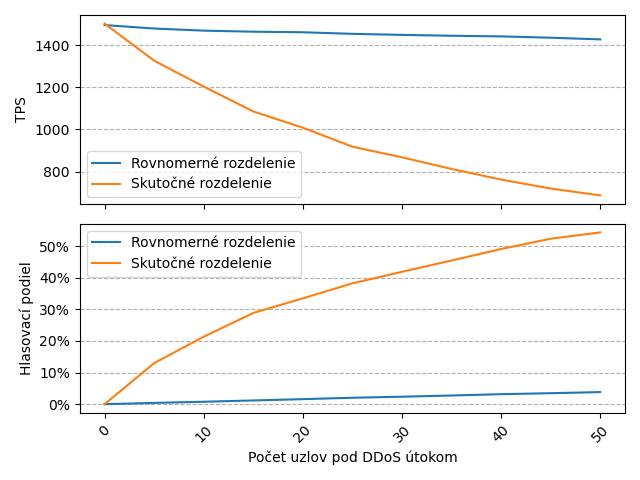
\includegraphics[width=.5\textwidth]{obrazky-figures/solana-scenario02}
	\caption{DDoS útok na najbohatšie (najvplyvnejšie) uzly v sieti.}
	\label{img:solana-scenario01}
\end{figure}

\subsection{Útok na dostupnosť lídrov}
Simulácia 10 epoch zo sieťou veľkou 1500 uzlov (rovnako ako skutočná sieť). Podiel zdrojov v simulovanej sieti je zhodný zo skutočným podielom v sieti. Rovnaká simulácia je spustená s DDoS útokom na najbohatšie uzly v sieti (postupne pre 5, 10, 15, 20 uzlov). Obrázok~\ref{img:solana-scenario02} zhrnuje výsledok tejto simulácie.
\begin{figure}[H]
	\centering
	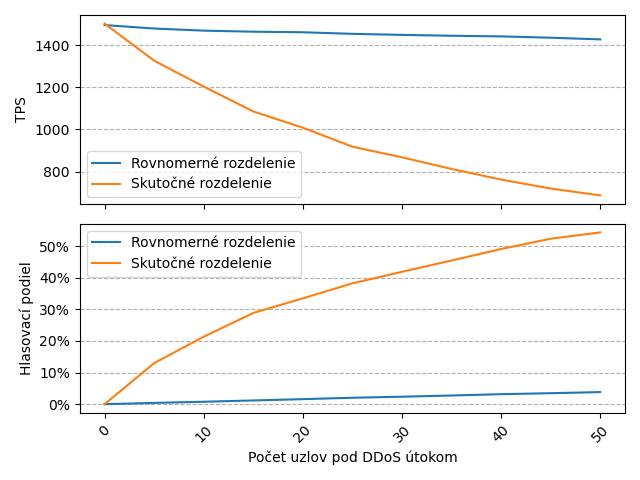
\includegraphics[width=.7\textwidth]{obrazky-figures/solana-scenario02}
	\caption{DDoS útok na najbohatšie (najvplyvnejšie) uzly v sieti.}
	\label{img:solana-scenario02}
\end{figure}

\section{Harmony}

Harmony zvyšuje svoju priepustnosť pomocou shardingu, ktorý by nemal znižovať bezpečnosť celého blockchainu. V následujúcej sekcii sú popísané výsledky simulácie shardingu.

\subsection{Sharding a bezpečnosť}\label{subsec:harmony-sec-exp}

V sekcii~\ref{subsec:harmony-sharding-sec} bola teoreticky analyzovaná bezpečnosť shardingu z hľadiska ovládnutia podskupiny uzlov útočníkom. Autori Harmony shardingu určili pravdepodobnosť ovládnutia shardu pomocou hypergeometrického rozdelenia, keďže distribúcia hlasovacieho podielu v podobe tokenov je určená skutočne pomocou neovplyvniteľného náhodného čísla. Avšak, tento výpočet uvažoval len podiel reprezentovaný pomocou tokenov a nie skutočný podiel. Tokenizácia podielu vnáša do distribúcie hlasovacieho práva v shardoch chybu. Druhým problémom tohoto dôkazu je, že autori uvažujú ideálnu distribúciu tokenov medzi shardy. Avšak takáto distribúcia bude v konečne veľkej sieti pre jednotlivé shardy vždy vykazovať nejakú chybu. Táto chyba rastie v priamej úmere k hodnote $\lambda$ (viď~\ref{subsec:harmony-token}). Dôvodom je, že z nastavenia $\lambda$ priamo vyplýva veľkosť jedného tokenu.

\begin{figure}[H]
	\centering
	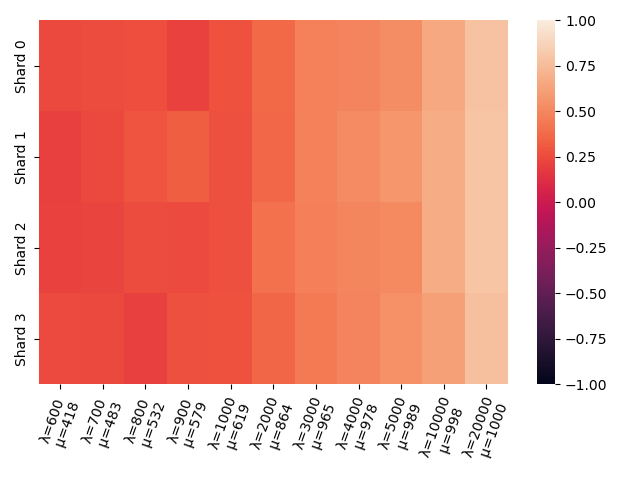
\includegraphics[width=\textwidth]{obrazky-figures/harmony/scenario01/shard-correlation.pdf}
	\caption{Teplotná mapa pre Spearmanov korelačný koeficient medzi skutočným podielom uzlov a hlasovacím právom jednotlivých shardoch v závislosti na hodnote $\lambda$.}
	\label{img:harmony-shard-correlation}
\end{figure}

Pre overenie bezpečnosti shardingu v sieti s veľkosťou 1000 uzlov a 4 shardy bola simulácia spúšťaná s rôznymi hodnotami $\lambda$. Pre potreby simulácie sa uvažovalo, že v každej epoche uzly vlastnili približne rovnaký podiel. Takéto rovnomerné rozdelenie hlasovacieho práva je ideálny bezpečnostný stav v PoS blockchaine. Simulácia sledovala skutočné rozdelenie hlasovacieho podielu medzi jednotlivé shardy v jednej epoche. Teplotná mapa na obrázoku~\ref{img:harmony-shard-correlation} zobrazuje v jednotlivých stĺpcoch výsledok simulácie pre konkrétne $\lambda$. Hodnota $\mu$ reprezentuje priemerný počet uzlov v jednej sharde pre dané $\lambda$ (môžeme vidieť, že $\mu$ rastie úmerne k veľkosti $\lambda$). Jednotlivé riadky ukazujú nameranú koreláciu medzi celkovým hlasovacím podielom a tým, ktorý bol skutočne pridelený uzlom v danej sharde. Na koreláciu bol použitý Spearmanov korelačný koeficient. Môžeme vidieť, že rastúce $\lambda$ zvyšuje podobnosť hlasovacieho podielu v shardoch voči skutočnému. V sekcii~\ref{label} bolo teoretický vypočítané, že pre 4 shardy je dostatočne bezpečné $\lambda=600$. Z teplotnej mapy je však vidieť, že hlasovací podiel v jednotlivých shardoch začína byť významne podobný skutočnému až pre $\lambda > 3000$. Avšak pri takto vysokej $\lambda$ sú v každej sharde takmer všetky uzly (pre $\lambda > 3000$ je $\mu \approx 1000$). Prítomnosť všetkých uzlov v každej sharde by však znemožnila akýkoľvek škálovatelnosť konsenzus protokolu.

\begin{figure}[H]
	\centering
	\includegraphics[width=\textwidth]{obrazky-figures/harmony/scenario01/byzantine280-shard-distribution.pdf}
	\caption{Hlasovací podiel byzantských uzlov v jednotlivých shardoch po dobu 1000 epoch. Červený predel určuje očakávaný podiel byzantských uzlov ($\frac{1}{3}$).}
	\label{img:harmony-byzantine-shard-distribution}
\end{figure}

Vyššie popísaný experiment ukázal nameranú nepresnosť podobnosti hlasovacieho podielu v shardoch a celkového podielu. Takáto odchýlka v distribúcii hlasovacieho práva znevýhodňuje poctivé uzly a poskytuje nepoctivým uzlom (ďalej len byzantské uzly) možnosť manipulovať s konsenzom. Nepresnosť v distribúcii hlasovacieho práva môže teoreticky spôsobiť to, že byzantské uzly síce vlastnia menej ako $\frac{1}{3}$ podielu, ale v niektorej sharde neprávom získajú viac ako $\frac{1}{3}$ podielu. V takom prípade môžu BFT konsenzus v danej sharde prekaziť. Pre určenie ako často by takýto scenár mohol nastať bola  vykonaná simulácia, ktorá uvažovala, že časť uzlov je byzantských. Simulácia bola opakovaná a množstvo byzantských uzlov bolo vždy zvýšené o 20. V prvom kole bol 200 s 1000 uzlov byzantských ($\frac{1}{4}$). V poslednom kole bolo 340 s 1000 uzlov byzantských (tesne pod $\frac{1}{3}$). V každej simulácii sa vykonalo 1000 epoch, a teda 1000 redistribúcii do shardov. Pre simuláciu bolo nastavené $\lambda$ na odporúčanú hodnotu 600. Obrázok~\ref{img:harmony-byzantine-shard-distribution} ukazuje výsledok simulácie, ak bolo 28\,\% uzlov byzantských. Červená čiara definuje teoretickú hodnotu podielu, ktorý by mali byzantské uzly spoločne v každej sharde vlastniť. Avšak rozptyl byzantského podielu okolo tejto hodnoty je pomerne vysoký. Z obrázka je vidieť, že ojedinele nastávajú aj prípady kedy v sharde byzantské uzly neprávom získajú $\geq \frac{1}{3}$. Tieto incidenty sú podrobnejšie zobrazené na obrázku~\ref{img:harmony-byzantine-shard-kde}, ktorý ukazuje histogram byzantského podielu v shardoch. Stredná hodnota hlasovacieho podielu je skutočne na 28\,\% avšak za dobu 1000 epoch sa až 156-krát stalo, že byzantské uzly neprávom získali dostatok hlasovacieho podielu na to aby znemožnili konsenzus. V týchto prípadoch bola až 5\,\% odchýlka hlasovacieho práva v neprospech poctivých uzlov. 

\begin{figure}[H]
	\centering
	\includegraphics[width=.5\textwidth]{obrazky-figures/harmony/scenario01/byzantine280-shard-kde.pdf}
	\caption{Histogram hlasovacieho podielu byzantských uzlov za 1000 epoch. Červene zvýraznená časť sú incidenty pri ktorých bol pridelený podiel v sharde väčší ako $\frac{1}{3}$.}
	\label{img:harmony-byzantine-shard-kde}
\end{figure}

\subsection{Sharding a priepustnosť}

V sekcii~\ref{subsec:harmony-sec-exp} boli vykonané simulačné experimenty, ktoré poukázali na to, že nastavenie parametru $\lambda$ na vyššiu hodnotu zvyšuje bezpečnosť shardingu. Tento parameter však ovplyvňuje aj priepustnosť blockchainu. Pre vyhodnotenie Harmony shardingu z hľadiska priepustnosti bola vykonaná simulácia siete o veľkosti 1000 uzlov a 4 shardy. Simulácia bola opakovaná postupne pre $\lambda \in \{200, 300, 400, ..., 2000\}$. V simulácii bolo uvažované, že veľkosť hlavičky každého bloku je 80\,B a jedna transakcia je veľká 32\,B. Simulácia ďalej predpokladala, že v sieti vzniká dostatok transakcií na to aby bolo možné do každého bloku v každej sharde pridať približne 500 nových transakcií.

\begin{figure}[H]
	\centering
	\begin{subfigure}{.5\textwidth}
		\centering
		\includegraphics[width=\linewidth]{obrazky-figures/harmony/scenario01/1000nodes-4shards-tps.pdf}
		\caption{Teoretická priepustnosť siete v TPS.}
		\label{img:harmony-scenario01-a}
	\end{subfigure}%
	\begin{subfigure}{.5\textwidth}
		\centering
		\includegraphics[width=\linewidth]{obrazky-figures/harmony/scenario01/1000nodes-4shards-transmit-stats.pdf}
		\caption{Skutočné množstvo prenesených dát v MB.}
		\label{img:harmony-scenario01-b}
	\end{subfigure}%
	\caption{Výsledok simulácie z hľadiska priepustnosti Harmony blockchainu.}
	\label{img:harmony-perform-exp}
\end{figure}

Výsledok simulácie sumarizuje obrázok~\ref{img:harmony-perform-exp}. ukazuje závislosť priepustnosti vzhľadom k $\lambda$. Z obrázku~\ref{img:harmony-scenario01-a} je vidieť, že ak je v danej sieti $\lambda = 300$, tak BC produkuje približne 2000 TPS. Taktiež môžeme vidieť, že ďalšie zvyšovanie $\lambda$ už priepustnosť nezvyšuje. Z hľadiska priepustnosti preto nie je dôvod aby bol parameter $\lambda$ nastavený na hodnotu väčšiu ako 300. Avšak, obrázok~\ref{img:harmony-scenario01-b} poukazuje na to, že ide len o teoretický graf pretože hlasovací protokol FBFT vyžaduje veľmi vysokú priepustnosť. Môžeme vidieť, že už pre $\lambda = 300$ je potrebné za jeden slot preniesť približne 750\,000 MB dát. Ak má slot 2 sekundy tak by musela sieť mať priepustnosť približne 400\,000 MB/s. Bežná 1 Gbps linka má priepustnosť 125MB/s. Je teda zrejmé, že v tejto konfigurácii siete by nebolo možné preniesť požadované dáta a konsenzus by sa nestihol uzniesť. Z hľadiska priepustnosti je teda nízka hodnota $\lambda$ výhodná.


\chapter{Záver}\label{chap:summary}

Táto práca sa zaoberala analýzou troch Proof-of-Stake protokolov pre uznesenie konsenzu (Harmony, Solana a Ouroboros). V~prvej časti práce boli tieto protokoly teoreticky zanalyzované a porovnané z~hľadiska bezpečnosti a výkonnosti.

Harmony a Solana sú založené na hlasovaní pomocou protokolu z~rodiny BFT. Hlasovacie právo a jeho významnosť závisí na množstve investovaných zdrojov (zabezpečenie pomocou Proof-of-Stake). Klasické BFT hlasovanie v~distribuovanej sieti má kvadratickú časovú zložitosť vzhľadom k~počtu uzlov siete. Harmony aj Solana zavádzajú modifikácie, ktoré pri rovnakej bezpečnosti umožňujú lineárnu škálovateľnosť vzhľadom k~počtu uzlov. Harmony ďalej používa na zvýšenie priepustnosti sharding, ktorý je odolný voči útoku ovládnutia konkrétneho shardu. Solana poskytuje oproti Harmony ešte väčšiu priepustnosť pomocou konceptu nazývaného Proof-of-History. Pre porovnanie, doba potrebná na vygenerovanie jedného bloku v~Harmony blockchaine je dostatočná na vytvorenie viac ako 400 nových blokov v~Solane. V~oboch protokoloch je kľúčová roľa vodcu, ktorý jediný môže pridávať nový blok do blockchainu. Vodca sa v~oboch protokoloch volí na krátke obdobie pomocou bezpečného a neovplyvniteľného hlasovania. Avšak, vodca je verejne známi a v~prípade jeho znefunkčnenia (napríklad pomocou DoS útoku) nie je možné pridávať žiaden nový obsah do blockchainu. Zraniteľnosť vodcu bola preto vyhodnotená ako potenciálna bezpečnostná slabina oboch protokolov.

Tretím analyzovaným protokolom je Ouroboros. Ten nepoužíva BFT hlasovanie, ale na uznesenie konsenzu používa pravidlo najdlhšieho reťazca (podobne ako Proof-of-Work protokol Bitcoin). Avšak na rozdiel od Bitcoinu, je tento protokol založený na koncepte Proof-of-Stake pretože nový blok môže vytvoriť len dopredu určený uzol. Tento uzol sa nazýva vodca a je zvolený pomocou distribuovanej náhodnej voľby, ktorú nie je možné ovplyvniť. Pritom platí, že čím väčšie množstvo zdrojov v~blockchaine uzol vlastní, tým väčšiu pravdepodobnosť má, že bude vodcom (koncpet Proof-of-Stake). Vytvorenie bloku nevyžaduje hlasovanie a teda jeho časová zložitosť vzhľadom k~počtu uzlov je konštantná. Na druhú stranu, Ouroboros neposkytuje okamžitú konzistenciu (na rozdiel od Harmony a Solana). Protokol je zabezpečený proti vytvoreniu alternatívneho reťazca, ktorý by bol potenciálne dlhší ako pôvodný.

V~druhej časti práce bude vytvorený model týchto troch protokolov, ktorý bude podrobený simulácii. Cieľom simulácie bude overiť bezpečnostné a výkonnostné parametre popísané v~prvej časti (prípadne odhaliť nové zraniteľnosti). Na simuláciu bude použitý už existujúci blockchain simulátor SimBlock, ktorý je pre potreby simulácie rozsiahlych Proof-of-Stake sietí najvhodnejší s~pomedzi dostupných blockchain simulátorov.

%===============================================================================
